\title{Implementing a MIPS processor using SME}
\author{Carl-Johannes Johnsen (grc421)}
%% Skabelon til LiCS-afleveringer

%%%%%%%%%%%%%%%%%%%%%%%%%%%%%%%%%%%%%%%%%%%%%%%%%%%%%%%%%%%%%%%
%% Begynd preamble
%%%%%%%%%%%%%%%%%%%%%%%%%%%%%%%%%%%%%%%%%%%%%%%%%%%%%%%%%%%%%%%
\documentclass[a4paper]{article}

%% Til at tegne træer!
\usepackage{tikz}
\usetikzlibrary{positioning,arrows,calc}
\tikzset{
    on grid,
    node distance=3cm,
    auto,
    block/.style = {
        draw,
        shape=rectangle,
        minimum height=3em,
        minimum width=3em,
        line width=1pt
    },
    control/.style = {
        draw,
        shape=circle,
        minimum height=7em,
        minimum width=3em,
        line width=1pt
    },
    mux/.style = {
        draw,
        shape=rectangle,
        minimum height=1.5em,
        minimum width=1em,
        line width=1pt
    },
    empty/.style = {
        shape=rectangle,
        minimum height=3em,
        minimum width=3em
    },
    >=latex',
}

%% Til at kunne have billeder
\usepackage{graphicx}
%% Til at kunne have source code
\usepackage{listings}
\lstset{
  breaklines=true,
  keepspaces=true,
  frame=ltrb,
  framesep=1pt,
  commentstyle=\color{Brown},
  basicstyle=\ttfamily\footnotesize,
  numbers=left,
  title=\lstname,
  columns=fullflexible,
  extendedchars=\true,
  inputencoding=ansinew,
}

%% Font and input encoding
%% Tillad æøå
\usepackage[T1]{fontenc}
\usepackage[utf8]{inputenc}
%% Babel (language)
\usepackage[UKenglish]{babel} % If you write in English
\usepackage[UKenglish]{isodate}
%\usepackage{parskip}
\usepackage{booktabs}
%\usepackage[danish]{babel} % Hvis du skriver på dansk

%% Til links
\usepackage{hyperref}
\usepackage{subfig}

%% AMS-Math packages
\usepackage{amsmath}
\usepackage{amssymb}
\usepackage{amsthm}
\newtheorem{theorem}{Theorem}
%% Extra symbols that we almost always need
\usepackage{stmaryrd}
\usepackage{color}
\usepackage{url}
\usepackage{semantic}
\usepackage{fancyref}
\usepackage{enumitem}

%%%%%%%%%%%%%%%%%%%%%%%%%%%%%%
%% Skift sidenumrene ud med X/total (lettere at rette :-)
\usepackage{lastpage}
\makeatletter
\renewcommand{\@oddfoot}{\hfil \thepage{}/\pageref{LastPage} \hfil}
\renewcommand{\@evenfoot}{\hfil \thepage{}/\pageref{LastPage} \hfil}
\makeatother
%%%%%%%%%%%%%%%%%%%%%%%%%%%%%%

% Til at få tabeller mindre?
\usepackage{adjustbox}

% Til klasse diagrammer
%\usepackage{pgf-umlcd}
%\renewcommand{\umldrawcolor}{black}
%\renewcommand{\umlfillcolor}{white}
%\let\classoperation\operation

% forkortelse af texttt!
\renewcommand{\bf}{\textbf}
\renewcommand{\tt}{\texttt}
\renewcommand{\sf}{\textsf}
\renewcommand{\it}{\textit}
\newcommand{\E}{\mathbb{E}}

% Forkortelser som bruger tt!
\newcommand{\tif}{\tt{ if }}
\newcommand{\tthen}{\tt{ then }}
\newcommand{\telse}{\tt{ else }}
\newcommand{\tfalse}{\tt{ false }}

%%%%%%%%%%%%%%%%%%%%%%%%%%%%%%%%%%%%%%%%%%%%%%%%%%%%%%%%%%%%%%%
%% Slut preamble -- herunder følger selve dokumentet!
%%%%%%%%%%%%%%%%%%%%%%%%%%%%%%%%%%%%%%%%%%%%%%%%%%%%%%%%%%%%%%%
\sloppy
\begin{document}
\maketitle

% TODO !!!
% Appendix
% Fix github

\begin{abstract}
    The Synchronous Message Exchange (SME) model, is a programming model, which
    closely resembles the CSP model and which is suitable for describing
    hardware. This thesis aims to combine the theory taught in a machine
    architecture class with the SME model, by implementing a MIPS processor
    using SME. I show how to construct the components of a MIPS processor as
    SME processes, and how to connect them by using SME busses. Furthermore, I
    show how to extend the processor, by introducing additional instructions
    and by pipelining the processor. Finally, I succesfully implement the
    Single Cycle and Pipelined MIPS processors onto an FPGA. \\

    \noindent
    Thesis supervisors: Brian Vinter and Kenneth Skovhede.
\end{abstract}

\newpage
\section*{Acknowledgements}
I would like to acknowledge my thesis supervisors Brian Vinter and Kenneth
Skovhede for guiding me through writing my thesis and through writing the
corresponding paper~\cite{ref:cpa-paper}. I would also like to thank the
employees in the eScience group at the Niels Bohr Institute, for taking their
time to listen to my project and give me feedback on my progress. Finally,
thanks to Daniel Lundberg Pedersen and Jeanette Johnsen for proof reading.

\newpage
\tableofcontents
\newpage

% \section*{Spørgsmål}
% \begin{enumerate}
%   \item Istedet for at have alle baggrunds teorien løbende, så tænkte jeg om der skulle
%     være et afsnit, som gennemgår al teorien?

%   \item Skal jeg have mere CSP teori med? I så fald medfører det vel også noget SME teori. - tjek intro

%   \item Skal jeg, og i så fald hvordan, referere min egen artikel? Eller skal jeg skynde mig at skrive den om, så de ikke er lig hinanden? - related work

%   \item Er det sidste afsnit om "Synthesizing" lidt for specifik?

%   \item Er de andre afsnit for uspecifikke?

%   \item Skal related work være et afsnit i introduction, eller skal det bare flettes ind i introduction? eller skal det et helt andet sted hen? Eget afsnit
% \end{enumerate}

% SME mangler!: Dobbelt tjek at de er med i rapporten, da det er nogle af de fund jeg har lavet!
% \begin{itemize}
%   \item AXI interface

%   \item Standard typer til top-level busser (pga block design ikke kan lide
%     custom typer)

%   \item Signal splitting

%   \item Caste et tal til en enum.
% \begin{lstlisting}
% control.opcode = (Opcode) ((instruction >> 26) & 0x3F);
% \end{lstlisting}
% skal lave VHDL:
% \begin{lstlisting}
% ControlIn_opcode <= SingleCycleMIPS_Opcodes'VAL(TO_INTEGER(UNSIGNED(instruction(31 downto 26))));
% \end{lstlisting}

%   \item Processer inde i klasser. Transpileren kan ikke lide navnene!
% \begin{lstlisting}
% public class ID
% {
%   public class Splitter : SimpleProcess
%   {
%   ...
% \end{lstlisting}

%   \item Lidt resikabelt at være ude i det, men muligheden for at kunne lave
%     noget, som kun kørte når clocken er høj, lav, rising edge eller falling edge?
%     Kunne f.eks. være noget ala OnHigh(). Lidt ligesom at det er lidt misvisende
%     at ikke clockede processer kalder det OnTick(), selv om der ikke er noget tick.

%   \item Der kan opstå fejl i Vivado, hvis man har et signal, som både skal gå
%     iblandt flere processer, men samtidig skal gå ud som top-level. Dette kan
%     fikses, ved at have et \texttt{signal} i den VHDL fil, som sørger for at
%     forbinde alt det indre, og at processerne så er forbundet til det signal,
%     istedet for andre forbindelser.
% \end{itemize}

\section{Introduction}
% TODO
Background and terminology for:

CSP

SME

Machine architecture

DIKU course

VHDL

C\#

%install monodevelop
%clone from github
%run process T4 template on SME.Render.VHDL/Entity.tt and
%SME.Render.VHDL/TopLevel.tt
%Open example project, and press f5 to build and run



% Remember! newpage on new chapters
%\newpage
%\section{Getting started with SME}
%Jeg tænkte, at der skulle være et afsnit her, som er lidt ligesom introduction, men mere ligesom en background. Dvs. tænkte, forklare CSP, MIPS, SME, Vivado osv. På den måde, så bliver de senere afsnit ikke ligeså tunge, da der er en masse der kan rykkes herop. Eller giver det ikke mening? 

\subsection{Installing required software for SME} Muligvis ryk alt det her ned
i appendix, da det mest bare er fifs?
monodevelop git
\subsection{Writing first SME program}
\subsection{C\# and bit hacking}
\subsection{Translating first SME program into VHDL}
\subsection{Running and verifying VHDL}


%\newpage
\section{Basic logic circuits}
\label{sec:logic-circuits}
In this section, we will be looking at some basic combinatorial circuits. We
use this as an entry point for hardware design, both due to the ARK
course\cite{ref:diku} at DIKU, and due to the book\cite{ref:ark} recommending
to read appendix C, which covers the basics of logic design, prior to reading
chapter 4, which covers implementing a simple MIPS processor. We are only going
to cover a subset of appendix C, as it should be sufficient as an introduction
to connecting simpler components together into a more complex network.

%TODO sig at det er fordi de andre ikke giver ny indsigt???

We start by looking at some logic gates, which implement some basic boolean
functions. Then we will combine these basic gates into more complex networks:
\begin{itemize}
    \item A decoder, which expands an $n$-bit input into $2^n$ outputs.
    \item A half adder, which takes two binary inputs and computes the sum and
        the carry of the two.
    \item A full adder, which does the same operation as the half adder, but
        with an additional third binary input.
    \item a $n$-bit adder, by combining a chain of a half adder followed by
        $n-1$ full adders.
\end{itemize}

For each of these combinatorial circuits, we go through the theory behind it,
describe the procedure of translating the theory into an SME network and
finally how to test and verify the SME networks.

\subsection{Basic logic gates}
A logic gate is a circuit abstraction, which has inputs and outputs, and
computes the logic function that corresponds to the gates name, i.e. its output
values are based upon the input values. We are going to implement the following
logic gates:

\begin{description}
    \item[\texttt{AND}] - outputs \texttt{1} iff. all of its inputs are
        \texttt{1}, otherwise it outputs \texttt{0}.

    \item[\texttt{OR}] - outputs \texttt{1} if one or more of its inputs are
        \texttt{1}, otherwise it outputs \texttt{0}.

    \item[\texttt{NOT}] - outputs the inverse of its input, i.e. \texttt{1}
        becomes \texttt{0} and \texttt{0} becomes \texttt{1}.

    \item[\texttt{XOR}] - outputs \texttt{1} iff exactly one of its inputs are
        \texttt{1}, otherwise it outputs \texttt{0}
\end{description}
The full truth table for all of the four logic gates with 2-bit input (except
for \texttt{NOT}, which only uses 1 bit) can be seen in Table
\ref{tab:truth-table}.

\begin{table}
    \centering
    \begin{tabular}{cc|cccc}
        \toprule
        \texttt{Bit1} & \texttt{Bit2} & \texttt{AND} & \texttt{OR} &
        \texttt{NOT} & \texttt{XOR} \\
        \midrule
        \texttt{0} & \texttt{0} & \texttt{0} & \texttt{0} & \texttt{1} &
            \texttt{0} \\
        \texttt{0} & \texttt{1} & \texttt{0} & \texttt{1} & \texttt{1} &
            \texttt{1} \\
        \texttt{1} & \texttt{0} & \texttt{0} & \texttt{1} & \texttt{0} &
            \texttt{1} \\
        \texttt{1} & \texttt{1} & \texttt{1} & \texttt{1} & \texttt{0} &
            \texttt{0} \\
        \bottomrule
    \end{tabular}
    \caption{The truth table for the four basic logic gates. Note: \texttt{NOT}
    is only considering \texttt{Bit1}.}
    \label{tab:truth-table}
\end{table}

\subsubsection*{Implementation}
Implementing each of these four logic gates is straightforward: There is an
input bus with two 1-bit values, a process for each of the gates, and an output
bus with a 1-bit value for each of the logic gates. We do not need additional
input busses, as each process which uses the bus as input, receives its own
copy of the input in each clock. Furthermore, we only need one output bus, as
each process writes to its own bit within it. Each process takes the two bits
from the input bus, computes their respective logical function and sends the
result out onto its bit on the output bus.

We could have made a more complex process, i.e. one that takes the two inputs,
and computes each function. This would reduce the amount of bus connections,
but we want to make each process as simple as possible, when constructing the
processor, as this makes arguing for correctness simpler.

\subsubsection*{Testing}
To ensure that the processes functions as expected, we construct a tester
process, which sets the bits on the input bus to all of the values in the truth
table, and checks whether or not each process puts the expected value from the
truth table onto their bit on the output bus. We use this testing technique, as
it tests the functionality of the processes, without knowing how they work
internally. We could also just have printed the output values, and verified the
results our selves, however automating this reduces the time needed for
verification. How the processes are connected can be seen in Figure
\ref{fig:logic-test}.

\begin{figure}
    \centering
    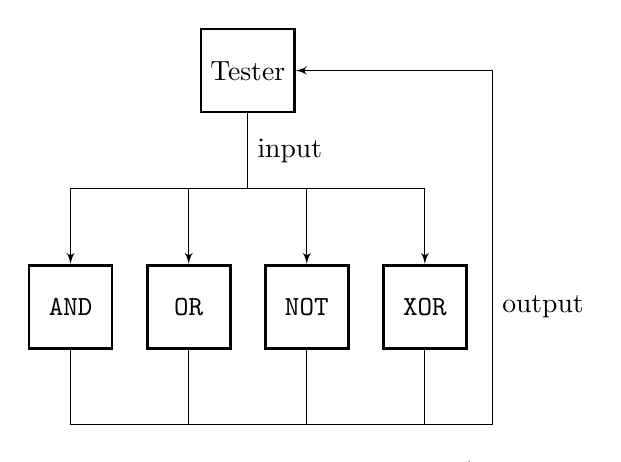
\begin{tikzpicture}[node distance=1.5cm]
        \node[block] (and) {\texttt{AND}};
        \node[block, right of=and] (or) {\texttt{OR}};
        \node[block, right of=or] (not) {\texttt{NOT}};
        \node[block, right of=not] (xor) {\texttt{XOR}};
        \node[above of=and] (input) at ($(or)!0.5!(not)$) {};
        \node[block, above of=input] (tester) {Tester};

        \path[-] (tester) edge node[midway, right] {input} (input.center);
        \path[draw, ->] (input.center) -| (and.north);
        \path[draw, ->] (input.center) -| (or.north);
        \path[draw, ->] (input.center) -| (not.north);
        \path[draw, ->] (input.center) -| (xor.north);

        \node[below of=and] (output) at ($(or)!0.5!(not)$) {};
        \node[right of=xor] (a) {output};

        \path[draw, -] (and.south) |- (output.center);
        \path[draw, -] (or.south) |- (output.center);
        \path[draw, -] (not.south) |- (output.center);
        \path[draw, -] (xor.south) |- (output.center);

        \path[draw, -] (output.center) -| (a.west);
        \path[draw, ->] (a.west) |- (tester.east);
    \end{tikzpicture}
    \caption{The structure of the test of the logic gates}
    \label{fig:logic-test}
\end{figure}

\subsection{Decoder}
A decoder is a component, which takes an $n$-bit input, and produces an
$2^n$-bit output, where the bit corresponding to the input numbers binary
representation is set to \texttt{1}. E.g. if the input value is the binary
representation of the number 5, then the 5th output bit will be \texttt{1}, and
the rest will be \texttt{0}.  Note: the output bits are zero indexed, i.e.
there is also an output bit for the binary representation of 0.

A decoder can be made from a set of \texttt{NOT} and \texttt{AND}
gates\cite{ref:logic}. We need to have $n$ \texttt{NOT} gates, and $2^n$
\texttt{AND} gates. For each input, we split it into two, and send the copy to
a \texttt{NOT} gate. Then for each output, we attach an \texttt{AND} gate, and
give it inputs corresponding to the binary representation of the number
%TODO mangler ord.
E.g. if we get the number 5, the binary representation is 101, i.e. the 5th
\texttt{AND} gate gets input from Bit0, \texttt{NOT} Bit1 and Bit2. An example
of a 2-bit decoder can be seen in Figure \ref{fig:2-bit-decoder}.

\begin{figure}
    \centering
    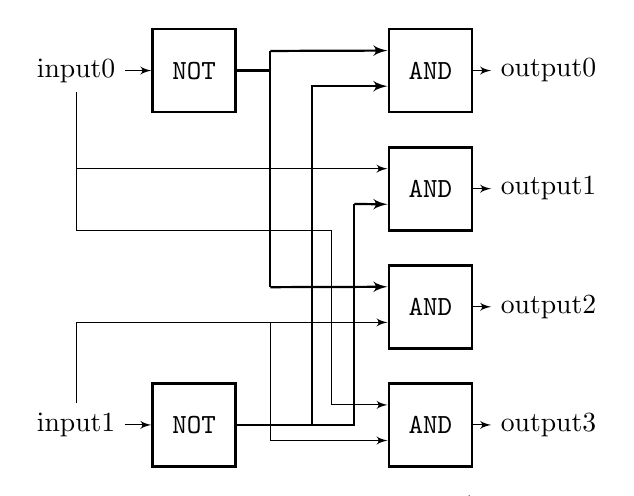
\begin{tikzpicture}[node distance=1.5cm]
        \node[block] (and0) {\texttt{AND}};
        \node[block, below of=and0] (and1) {\texttt{AND}};
        \node[block, below of=and1] (and2) {\texttt{AND}};
        \node[block, below of=and2] (and3) {\texttt{AND}};

        \node[right of=and0] (output0) {output0};
        \node[right of=and1] (output1) {output1};
        \node[right of=and2] (output2) {output2};
        \node[right of=and3] (output3) {output3};

        \path[draw, ->] (and0) -- (output0);
        \path[draw, ->] (and1) -- (output1);
        \path[draw, ->] (and2) -- (output2);
        \path[draw, ->] (and3) -- (output3);

        \node[empty, left of=and0] (andinp0) {};
        \node[empty, left of=and1] (andinp1) {};
        \node[empty, left of=and2] (andinp2) {};
        \node[empty, left of=and3] (andinp3) {};

        \node[block, left of=andinp0] (not0) {\texttt{NOT}};
        \node[block, left of=andinp3] (not1) {\texttt{NOT}};

        \node[left of=not0] (input0) {input0};
        \node[left of=not1] (input1) {input1};

        \path[draw, ->] (input0) -- (not0);
        \path[draw, ->] (input1) -- (not1);

        \path[draw, thick, -] (not0) -| (andinp0.155);
        \path[draw, thick, ->] (andinp0.155) -- (and0.155);
        \path[draw, thick, -] (not1.east) -| (andinp0.south);
        \path[draw, thick, ->] (andinp0.south) |- (and0.200);

        \path[draw, ->] (input0) |- (and1.155);
        \path[draw, thick, -] (not1.east) -| (andinp1.340);
        \path[draw, thick, ->] (andinp1.340) -- (and1.200);

        \path[draw, thick, -] (not0.east) -| (andinp2.155);
        \path[draw, thick, ->] (andinp2.155) -- (and2.155);
        \path[draw, ->] (input1.north) |- (and2.200);

        \path[draw, -] (input0) |- (andinp1.295);
        \path[draw, ->] (andinp1.295) |- (and3.155);
        \path[draw, -] (input1) |- (andinp2.200);
        \path[draw, ->] (andinp2.200) |- (and3.200);

    \end{tikzpicture}
    \caption{An 2-bit decoder made by \texttt{AND} and \texttt{NOT} gates.}
    \label{fig:2-bit-decoder}
\end{figure}

\subsubsection*{Implementation}
To implement a 2-bit decoder, we just need to connect logic gate processes,
which we already have. How to connect a 2-bit decoder can be seen in Figure
\ref{fig:2-bit-decoder}.

We could have made the decoder a single process, but we are trying to emphasize
connecting multiple processes together, in order to gain functionality.

However, making a scalable decoder is not trivial, as SME requires everything
to be known at compile time, and we cannot make a generic process, as these
depend on the names of the different busses. To solve this problem, we can use
C\# templates. For each input bit, we create an input bus. Then, for each input
bus, we create an \texttt{NOT} gate process, which takes the input bus
corresponding to its index. Then, we create $2^n$ output busses, and for each
of these, we connect an \texttt{AND} gate with its corresponding output bus.
Finally, for each of these \texttt{AND} gates, we connect the busses whose
logical \texttt{AND} will produce a \texttt{1}. E.g. for \texttt{output0}, we
connect all the busses from all of the \texttt{NOT} gates, for
\texttt{output1}, we connect all the \texttt{NOT} gates, except from the bus
from the first \texttt{NOT} gate, as this should be the first input bus.

\subsubsection*{Testing}
To test the 2-bit decoder, we follow the same procedure as with the logic
gates. We construct a tester process, which sends input to the logic gates, and
verifies the output from the \texttt{AND} gates. This is also what we need to
do with the $n$-bit decoder. However as with the $n$-bit decoder, we are going
to need C\# templates, as the tester process also needs a variable amount of
busses. Each of the two tester processes should send all possible inputs as
input.

\subsection{Adder}
An adder is an component, which adds two binary numbers together. As with the
decoder, an adder can be constructed by a combination of \texttt{AND},
\texttt{OR} and \texttt{XOR} gates\cite{ref:logic}. An $n$-bit adder is a chain
of two major components: an half adder and a full adder.

The half adder is the initial component in the chain. It takes two binary
inputs, and outputs the sum and the carry of the addition (See Figure
\ref{fig:half-adder}). The rest of the $n$-bit adder consists of a chain of
full adders, that take three inputs, A, B, and the carry from the previous link
in the chain, and outputs the sum and the carry of the addition (See Figure
\ref{fig:full-adder}). The combination of the components can be seen in Figure
\ref{fig:n-bit-adder}.

\begin{figure}
    \centering
    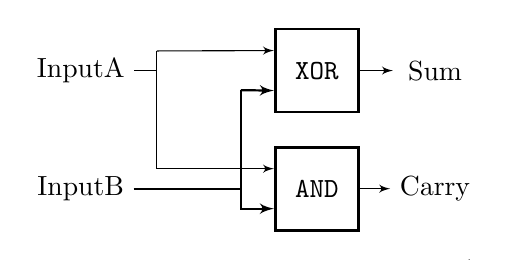
\begin{tikzpicture}[node distance=1.5cm]
        \node[block] (xor) {\texttt{XOR}};
        \node[block, below of=xor] (and) {\texttt{AND}};

        \node[empty, left of=xor] (xorin) {};
        \node[empty, left of=and] (andin) {};

        \node[left of=xorin] (inputa) {InputA};
        \node[left of=andin] (inputb) {InputB};

        \node[empty, right of=xor] (sum) {Sum};
        \node[empty, right of=and] (carry) {Carry};

        \path[draw, -] (inputa) -| (xorin.155);
        \path[draw, ->] (xorin.155) -- (xor.155);
        \path[draw, ->] (xorin.west) |- (and.155);

        \path[draw, thick, -] (inputb.east) -| (xorin.335);
        \path[draw, thick, ->] (xorin.335) -- (xor.205);
        \path[draw, thick, ->] (andin.east) |- (and.205);

        \path[draw, ->] (xor) -- (sum);
        \path[draw, ->] (and) -- (carry);
    \end{tikzpicture}
    \caption{An half adder composed of \texttt{XOR} and \texttt{AND} gates}
    \label{fig:half-adder}
\end{figure}

\begin{figure}
    \centering
    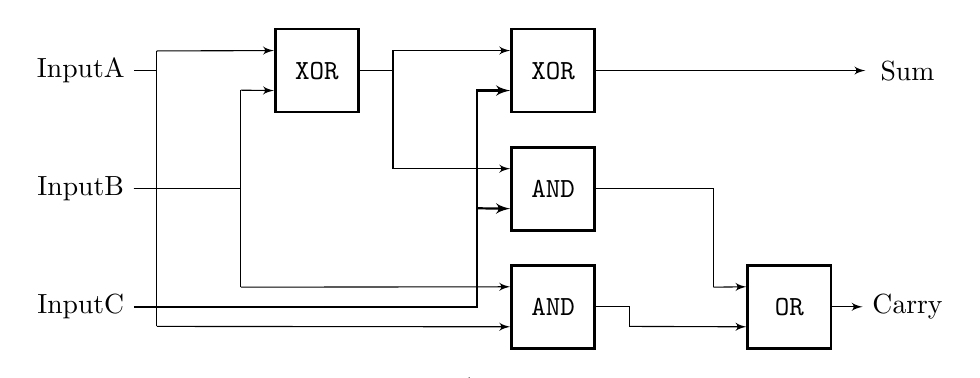
\begin{tikzpicture}[node distance=1.5cm]
        \node[block] (or) {\texttt{OR}};
        \node[empty, left of=or] (orin) {};
        \node[block, left of=orin] (and1) {\texttt{AND}};
        \node[block, above of=and1] (and0) {\texttt{AND}};
        \node[empty, left of=and0] (and0in) {};
        \node[block, above of=and0] (xor1) {\texttt{XOR}};
        \node[empty, left of=xor1] (xor1in) {};
        \node[block, left of=xor1in] (xor0) {\texttt{XOR}};
        \node[empty, left of=xor0] (xor0in) {};
        \node[empty, left of=xor0in] (inputa) {InputA};
        \node[empty, below of=inputa] (inputb) {InputB};
        \node[empty, below of=inputb] (inputc) {InputC};
        \node[empty, right of=inputc] (inputcout) {};
        \node[empty, right of=xor1] (sum) {};
        \node[empty, right of=sum] (summ) {};
        \node[empty, right of=summ] (summm) {Sum};
        \node[empty, right of=or] (carry) {Carry};

        \path[draw, -] (inputa.east) -| (xor0in.155);
        \path[draw, ->] (xor0in.155) -- (xor0.155);
        \path[draw, -] (inputb.east) -| (xor0in.335);
        \path[draw, ->] (xor0in.335) -- (xor0.205);

        \path[draw, -] (inputa.east) -| (inputcout.205);
        \path[draw, ->] (inputcout.205) -- (and1.205);
        \path[draw, -] (inputb.east) -| (inputcout.25);
        \path[draw, ->] (inputcout.25) -- (and1.155);

        \path[draw, thick, -] (inputc.east) -| (and0in.335);
        \path[draw, thick, ->] (and0in.335) -- (and0.205);
        \path[draw, thick, ->] (and0in.335) |- (xor1.205);

        \path[draw, -] (xor0.east) -- (xor1in.west);
        \path[draw, ->] (xor1in.west) |- (xor1.155);
        \path[draw, ->] (xor1in.west) |- (and0.155);

        \path[draw, -] (and1.east) -| (orin.205);
        \path[draw, ->] (orin.205) -- (or.205);
        \path[draw, ->] (xor1) -- (summm);
        \path[draw, -] (and0.east) -| (orin.25);
        \path[draw, ->] (orin.25) -- (or.155);
        \path[draw, ->] (or) -- (carry);
    \end{tikzpicture}
    \caption{A full adder composed of \texttt{AND}, \texttt{OR} and
    \texttt{XOR} gates}
    \label{fig:full-adder}
\end{figure}

\begin{figure}
    \centering
    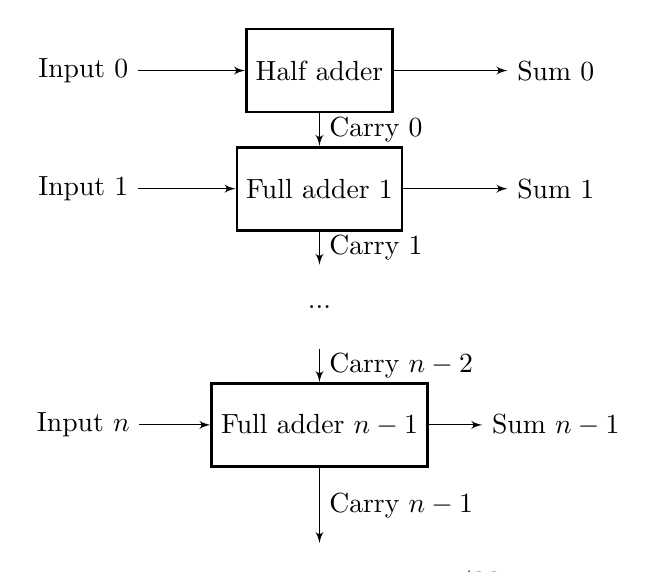
\begin{tikzpicture}[node distance=1.5cm]
        \node[block] (half) {Half adder};
        \node[block, below of=half] (full1) {Full adder 1};
        \node[empty, below of=full1] (dot) {...};
        \node[block, below of=dot] (fulln) {Full adder $n-1$};

        \node[empty, left of=half] (spacingl) {};
        \node[empty, right of=half] (spacingr) {};

        \node[empty, left of=spacingl] (in0) {Input 0};
        \node[empty, below of=in0] (in1) {Input 1};
        \node[empty, below of=in1] (vertspacel) {};
        \node[empty, below of=vertspacel] (inn) {Input $n$};

        \node[empty, right of=spacingr] (out0) {Sum 0};
        \node[empty, below of=out0] (out1) {Sum 1};
        \node[empty, below of=out1] (vertspacer) {};
        \node[empty, below of=vertspacer] (outn) {Sum $n-1$};
        \coordinate[below of=fulln] (carry);

        \path[draw, ->] (in0) -- (half);
        \path[draw, ->] (in1) -- (full1);
        \path[draw, ->] (inn) -- (fulln);

        \path[draw, ->] (half) -- (out0);
        \path[draw, ->] (full1) -- (out1);
        \path[draw, ->] (fulln) -- (outn);

        \path[draw, ->] (half) -- node [midway, right] {Carry 0} (full1);
        \path[draw, ->] (full1) -- node [midway, right] {Carry 1} (dot);
        \path[draw, ->] (dot) -- node [midway, right] {Carry $n-2$} (fulln);
        \path[draw, ->] (fulln) -- node [midway, right] {Carry $n-1$} (carry);
    \end{tikzpicture}
    \caption{An $n$-bit adder composed of a half adder, and $n-1$ full adders.
    Note: Input A and B are both inside the inputs for simplicity.}
    \label{fig:n-bit-adder}
\end{figure}

\subsubsection*{Implementation}
The half adder and the full adder is made like the decoder, in which we have
the basic logic gate processes, and connect them as specified in Figure
\ref{fig:half-adder} and Figure \ref{fig:full-adder}.

To make the $n$-bit adder, we have to use C\# templates like we did when
constructing the $n$-bit decoder. We program it so that each of the input bits
has its own bus, each of the output sums has its own bus, and each of the
carrys have their own bus. Then we start by making a half adder, which has the
inputs: input A bit 0 and input B bit 0. The initial half adder outputs its sum
on sum 0, and outputs the carry on carry 0. Then we construct $n-1$ full
adders, where full adder $i$ (1-indexed) has the inputs: input A bit $i$, input
B bit $i$ and carry $i-1$. Each full adder has output $i$ and carry $i$ as
output.

\subsubsection*{Testing}
To test the adder, we construct a tester process as before. We start by testing
the two subcomponents, the half and the full adder, by giving each every
possible input, and verifying the output. For the $n$-bit adder, we make a
function that takes an integer as input, and sends it along the corresponding
input wires. We also make a similar function that takes the values from the
output wires and packs it into an integer. This makes the test more human
readable, and reduces the chance of failure, when hand encoding/decoding binary
numbers. There are two tests: the simplest addition: 2+2, adding two numbers
together that produce an overflow and finally a series of adding random
numbers together.


%\newpage
\section{Core components}
\label{sec:components}
\subsection{Register file}
The register file is the component that holds values for the processor. It is
the first step in a memory hierarchy, and thus the fastest memory available.
There are 32 registers in a 32-bit MIPS processor. The registers are devided
into groups based on their usage. This does not matter from a hardware
perspective, except for register 0, which is immutable and always 0.

A register file has 5 inputs: Read address A, Read address B, Write enabled,
Write address and Write data. It also has two outputs: Output A and Output B.
We need to be careful of the order in which we read and write from the register
file. We need to make sure that when an instruction reads from the register
file, it always gets the latest data, i.e. if an instruction reads from the
same register as a previous instruction writes to, it should get the written
value. This is easy to fix in the single cycle processor, as we just need to
write before reading.

\begin{figure}
    \centering
    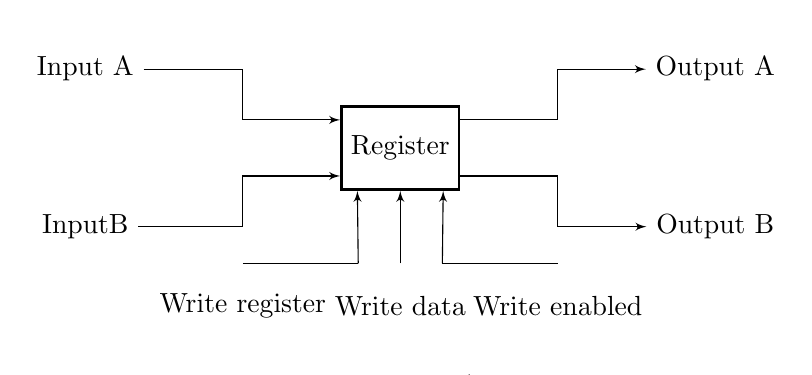
\begin{tikzpicture}[node distance=2cm]
        \node[empty] (inputa) {Input A};
        \node[empty, below of=inputa] (inputb) {InputB};

        \node[empty, right of=inputa] (spacing) at ($(inputa)!0.5!(inputb)$) {};
        \node[block, right of=spacing] (register) {Register};
        \node[empty, below of=register] (writedata) {Write data};
        \node[empty, left of=writedata] (write) {Write register};
        \node[empty, right of=writedata] (writeenabled) {Write enabled};

        \node[empty, right of=inputa] (space) {};
        \node[empty, right of=space] (spacee) {};
        \node[empty, right of=spacee] (spaceee) {};
        \node[empty, right of=spaceee] (outputa) {Output A};
        \node[empty, below of=outputa] (outputb) {Output B};
        \node[empty, left of=outputb] (bspace) {};

        \path[draw, -] (inputa) -| (spacing.north);
        \path[draw, ->] (spacing.north) |- (register.155);
        \path[draw, -] (inputb) -| (spacing.south);
        \path[draw, ->] (spacing.south) |- (register.205);

        \path[draw, -] (write) |- (writedata.135);
        \path[draw, ->] (writedata.135) -- (register.225);
        \path[draw, ->] (writedata) -- (register);
        \path[draw, -] (writeenabled) |- (writedata.45);
        \path[draw, ->] (writedata.45) -- (register.315);

        \path[draw, -] (register.335) -| (bspace.north);
        \path[draw, ->] (bspace.north) |- (outputb);
        \path[draw, -] (register.25) -| (spaceee.south);
        \path[draw, ->] (spaceee.south) |- (outputa);
    \end{tikzpicture}
    \caption{The register file}
    \label{fig:register}
\end{figure}

\bf{Testing} - I start by testing if some of the initial values of the register
file is correctly set to 0. Then I test if I can write to a register, and
whether or not I can read the same value from the same address in the register.
Then, I try to write to all of the registers, except for 0, and check whether
or not the output that I get, corresponds with the output that I wrote.

\subsection{ALU}
The ALU (Arithmetic Logic Unit) is the part of the processor, which makes the
actual computation. It takes three inputs: InputA, InputB and an ALU opcode
indicating which computation to perform. It has two outputs: The result of the
computation, and a zero flag indicating whether or not the result of the
computation was 0.

I follow the approach from the book % TODO ref!
and have implemented the basic processor operations: \texttt{add}, \texttt{sub},
\texttt{and}, \texttt{or} and \texttt{slt} (set less than).

I have tested each of the four operations.


%\newpage
\section{Single cycle MIPS processor}
\label{sec:single-cycle}
In this section, we will be combining the core components into a single cycle
MIPS processor, i.e. a processor where exactly one instruction is executed per
clock cycle. When it is in place, we will be writing the first program, and
compiling it into the processor, and running it.

Following the single cycle MIPS processor, we will be extending
the processor so that it can handle more instructions. Along each added
instruction, we will be extending our first program, in order to verify that
the added instruction works.

Finally, we will be writing two larger programs, and look into compiling them
into a series of hex values, that we can copy straight into the Instruction
Memory.

\subsection{Wiring up the processor}
\begin{figure}
    \centering
    \scalebox{0.5}{
        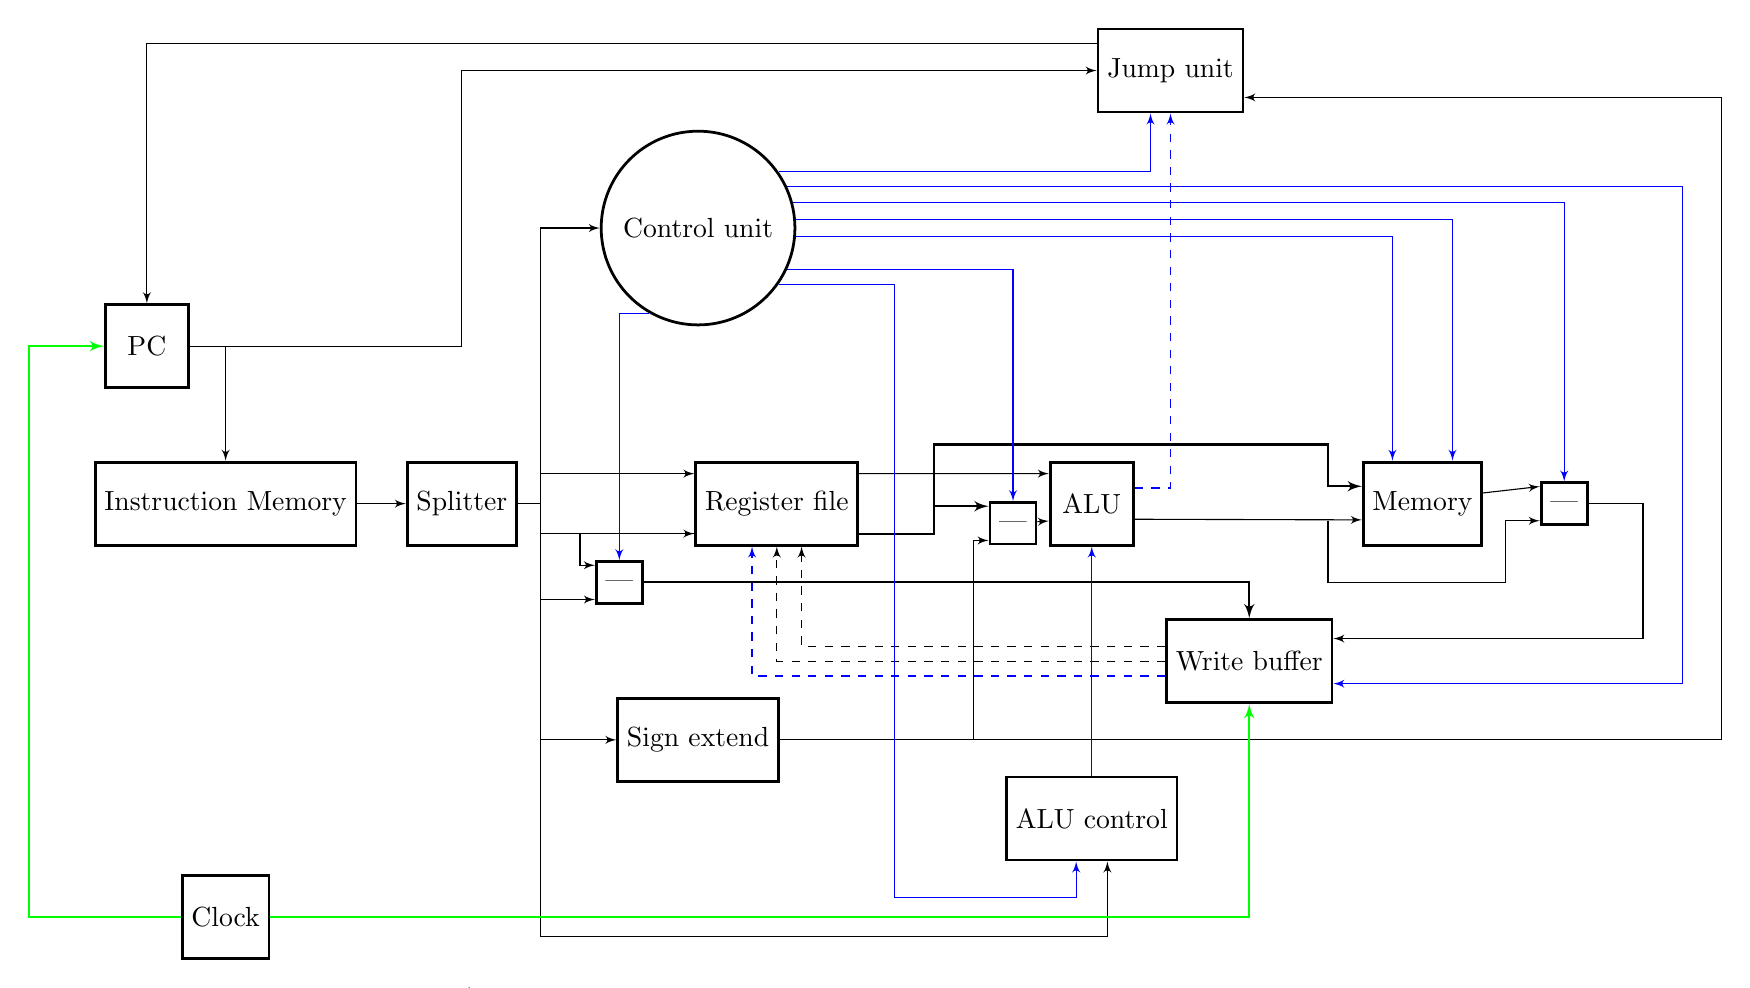
\begin{tikzpicture}
            \node[block] (reg) at (0,0) {Register file};
            \node[control] (cont) at (-1,3.5) {Control unit};
            \node[block] (jump) at (5,5.5) {Jump unit};
            \node[empty] (splitspace) at (-3,0) {};
            \node[block] (split) at (-4,0) {Splitter};
            \node[block] (if) at (-7,0) {Instruction Memory};
            \node[block] (sign) at (-1,-3) {Sign extend};
            \node[block] (alu) at (4,0) {ALU};
            \node[block] (alucont) at (4,-4) {ALU control};
            \node[block] (mem) at (8.2,0) {Memory};
            \node[mux] (memread) at (10,0) {|};
            \node[mux] (imm) at (3, -0.25) {|};
            \node[mux] (regdst) at (-2,-1) {|};
            \node[block] (pc) at (-8, 2) {PC};
            \node[block] (writebuf) at (6, -2) {Write buffer};

            \path[draw, ->] (if) -- (split);
            \path[draw, -] (split) -- (splitspace.center);
            \path[draw, ->] (splitspace.center) |- (sign);
            \path[draw, ->] (splitspace.center) |- (cont);
            \path[draw, ->] (splitspace.center) |- (reg.160);
            \path[draw, ->] (splitspace.center) |- (reg.200);
            %\path[draw, ->] (splitspace.center) |- (alucont.200);
            \path[draw, ->] (splitspace.center) |- (2,-5.5) -| (alucont.290);
            \path[draw, ->] (splitspace.center) |- (regdst.215);
            \path[draw, ->] (reg.200) -| (-2.5, -0.5) |- (regdst.145);
            %\path[draw, ->] (alucont) -| (12.5, 0) |- (jump);
            \path[draw, thick, ->] (reg.340) -| (2,-0.25) |- (imm.145);
            \path[draw, thick, ->] (2,-0.25) |- (3,0.75) -- (7,0.75) |-
            (mem.164);
            \path[draw, ->] (reg.20) -- (alu.145);
            \path[draw, ->, dashed, color=blue] (alu.20) -| (jump);
            %\path[draw, ->] (alu.340) -- (jal);
            %\path[draw, ->] (jal) -- (mem.196);
            %\path[draw, ->] (jal) -- (writebuf);
            \path[draw, ->] (alu.340) -- (mem.195);
            \path[draw, ->] (imm) -- (alu.202);
            \path[draw, ->] (7, -0.22) |- (8, -1) -| (9.25,-0.5) |-
            (memread.215);
            \path[draw, ->] (mem.10) -- (memread.145);
            \path[draw, ->] (sign) -| (2.5, -1) |- (imm.215);
            \path[draw, ->] (2.5,-3) -| (12, 0) |- (jump.340);
            %\path[draw, thick, ->] (regdst) -| (5, -0.6) |- (jal.210);
            \path[draw, thick, ->] (regdst) -| (writebuf);
            \path[draw, ->] (pc) -| (if);
            \path[draw, ->] (pc) -| (-4, 4) |- (jump);
            \path[draw, ->] (jump.160) -| (pc);
            \path[draw, ->] (memread) -| (11, -1) |- (writebuf.15);
            \path[draw, dashed, ->] (writebuf.170) -| (reg.300);
            \path[draw, dashed, ->] (writebuf) -| (reg);
            \path[draw, dashed, ->, color=blue] (writebuf.190) -| (reg.240);

            \path[draw, ->, color=blue] (alucont) -- (alu);
            \path[draw, ->, color=blue] (cont.35) -| (jump.245);
            \path[draw, ->, color=blue] (cont.25) -| (11.5,0) |-
            (writebuf.345);
            \path[draw, ->, color=blue] (cont.15) -| (memread);
            \path[draw, ->, color=blue] (cont.5) -| (mem.55);
            \path[draw, ->, color=blue] (cont.355) -| (mem.125);
            \path[draw, ->, color=blue] (cont.335) -| (imm);
            \path[draw, ->, color=blue] (cont.325) -| (1.5, -4) |-
            (2, -5) -| (alucont.250);
            \path[draw, ->, color=blue] (cont.240) -| (regdst);

            \node[block] (clock) at (-7, -5.25) {Clock};
            \path[draw, ->, thick, color=green] (clock) -| (-9.5,0) |- (pc);
            \path[draw, ->, thick, color=green] (clock) -| (writebuf);
        \end{tikzpicture}
    }
    \caption{Simple single cycle MIPS processor. The units with | indicate
    multiplexors. The Clock is not an SME process, but has been added to
    emphasize which processes that are clocked.}
    \label{fig:simple-full}
\end{figure}
With all the components in place, wiring up the single cycle MIPS processor is
straightforward. We just need to declare the busses with the corresponding
names, and then SME handles the wiring process. Note that as previously
mentioned, the Write Buffer and the PC register should be clocked processes.
The wiring of the single cycle MIPS processor can be seen in Figure
\ref{fig:simple-full}.

\subsection{Writing the first program}
As mentioned before, the first single cycle MIPS processor should be able to
handle \texttt{add}, \texttt{sub}, \texttt{and}, \texttt{or}, \texttt{slt},
\texttt{sw}, \texttt{lw} and \texttt{beq}. As such, the first program should
consist of these. The program and the different parts of each of the
instructions can be seen in Table \ref{tab:first-program}.
\begin{table}
    \centering
    \begin{tabular}{rllllllll}
        \toprule
        Address & Instruction & opcode & rs & rt & rd/imm & shmt & funct & hex \\
        \midrule
        \texttt{0x00} & \texttt{add \$3 \$1 \$2} & \texttt{0x00} &
        \texttt{0x01} & \texttt{0x02} & \texttt{0x03} & \texttt{0x00} &
        \texttt{0x20} & \texttt{0x00221820} \\ % 5 + 2 = 7

        \texttt{0x04} & \texttt{sub \$4 \$3 \$2} & \texttt{0x00} &
        \texttt{0x03} & \texttt{0x02} & \texttt{0x04} & \texttt{0x00} &
        \texttt{0x22} & \texttt{0x00622022} \\ %  7 - 2 = 5

        \texttt{0x08} & \texttt{and \$5 \$3 \$1} & \texttt{0x00} &
        \texttt{0x03} & \texttt{0x03} & \texttt{0x05} & \texttt{0x00} &
        \texttt{0x24} & \texttt{0x00612824} \\ % 7 and 5 = 5

        \texttt{0x0C} & \texttt{and \$6 \$3 \$1} & \texttt{0x00} &
        \texttt{0x03} & \texttt{0x03} & \texttt{0x06} & \texttt{0x00} &
        \texttt{0x25} & \texttt{0x00613025} \\ % 7 or 5 = 7

        \texttt{0x10} & \texttt{slt \$7 \$6 \$5} & \texttt{0x00} &
        \texttt{0x06} & \texttt{0x05} & \texttt{0x07} & \texttt{0x00} &
        \texttt{0x2A} & \texttt{0x00C5382A} \\ % 7 < 5 = 1

        \texttt{0x14} & \texttt{sw \$6  0x0(\$0)} & \texttt{0x2B} &
        \texttt{0x00} & \texttt{0x06} & \texttt{0x0000} & - &
        - & \texttt{0xAC060000} \\ % M[0] = 7

        \texttt{0x18} & \texttt{lw \$8  0x0(\$0)} & \texttt{0x23} &
        \texttt{0x00} & \texttt{0x07} & \texttt{0x0000} & - &
        - & \texttt{0x8C070000} \\ % $8 = M[0] (= 7)

        \texttt{0x1C} & \texttt{beq \$5 \$4 0x4} & \texttt{0x04} &
        \texttt{0x05} & \texttt{0x04} & \texttt{0x0004} & - &
        - & \texttt{0x10A40004} \\ % if 5 == 5 then skip next

        \texttt{0x20} & \texttt{add \$9 \$8 \$6} & \texttt{0x00} &
        \texttt{0x08} & \texttt{0x06} & \texttt{0x09} & \texttt{0x00} &
        \texttt{0x20} & \texttt{0x01064820} \\ % 7 + 7 = 14 // should not run!

        \texttt{0x24} & \texttt{add \$10 \$8 \$6} & \texttt{0x00} &
        \texttt{0x08} & \texttt{0x06} & \texttt{0x0A} & \texttt{0x00} &
        \texttt{0x20} & \texttt{0x01065020} \\ % 7 + 7 = 14
        \bottomrule
    \end{tabular}
    \caption{The first MIPS program. Note that the instruction at \texttt{0x20}
    should be skipped due to the \texttt{beq} at \texttt{0x1C}.}
    \label{tab:first-program}
\end{table}

%TODO lav om til at læse fra en binary fil!
Inserting this program into the Instruction Memory is straightforward: just
create an \texttt{byte} array, which is initialized to the hex values from the
instruction column in Table \ref{tab:first-program}. Since we do not have any
way of feeding values into the Register File at this moment, we are going to
hardcode registers 1 and 2 with the values 5 and 2 respectively. When the
program has finished, the contents of the register file should be as in Table
\ref{tab:first-result}.
\begin{table}
    \centering
    \begin{tabular}{rrrrrrrrrrrrrrrrrrrr}
        \toprule
        Address & 0 & 1 & 2 & 3 & 4 & 5 & 6 & 7 & 8 & 9 & 10 \\
        \midrule
        Value & 0 & 5 & 2 & 7 & 5 & 5 & 7 & 1 & 7 & 0 & 14 \\
        \bottomrule
    \end{tabular}
    \caption{The register file after the first program has finished.}
    \label{tab:first-result}
\end{table}

\subsection{Extending the accepted instruction set}
\subsubsection*{Additional simple R format instructions}
The simplest instructions to add, are the remaining simple R format
instructions. These are \texttt{addu}, \texttt{subu}, \texttt{xor},
\texttt{nor} and \texttt{sltu}. The only modifications are to extend the ALU
Operation \texttt{enum}, and then add the remaining cases in the ALU Control
and the ALU. As described in section \ref{sec:alu}, it is important to cast the
input \texttt{uint} to \texttt{int} before making the computation, if the
operation is signed.

To test each of these instructions, we can just append them to our initial
program.

\subsubsection*{Immediate instructions}
The next instruction we want to add is the \texttt{ori} instruction, as this
would allow us to feed values into the processor without hardcoding it. While
we are doing this, we should also add \texttt{addi}, \texttt{addiu},
\texttt{slti}, \texttt{sltiu}, \texttt{andi} and \texttt{xori}, as these
requires the same amount of work.

For the logical immediates, it is important, that the Sign Extend does not
sign extend. As such, we add another signal to the Control Unit:
\texttt{LogicalImmediate}, which goes to the Sign Extend. The Sign Extend
should then, in the case the \texttt{LogicalImmediate} flag is \texttt{1}, cast
its input as \texttt{unsigned}, such that any potential sign bits are not
extended. Then we just need to extend the opcode and ALUOp \texttt{enum}, and
add the remaining \texttt{case}s in the Control Unit and the ALU Control.

Once the processor have been extended, we can prepend instructions at the
beginning of the program. Furthermore, we can remove our previous hardcoding of
initial values in the Register File.

\subsubsection*{Jump instruction}
We are going to introduce another format: the J format. This format is used for
executing the \texttt{j} instruction. The first step is to extend the Splitter,
as it should now send the lower 26 bits to the Jump Unit. Then the Control Unit
should be extended, both in the opcode \texttt{enum}, and it should have another
control signal output: \texttt{jump}, which should be connected to the Jump
Unit.

Finally, the Jump Unit should be extended. It should take the 26 bits from the
Splitter, and left shift it by 2, such that it becomes a 28 bit number. Then,
it should take the 4 most significant bits from the PC+4, and prepend them to
the extended number.  Finally, we are going to add a multiplexor, which takes
this newly computed address, the previous output address, and the \texttt{jump}
control signal. If the control signal is \texttt{0}, then the original output
should be output, otherwise the newly computed jump address.

Then the program can be extended with a \texttt{j} instruction, in the same
manner as the \texttt{beq} instruction was tested before, i.e. trying to jump
over some instructions.

\subsubsection*{Branching instructions}
Then we are going to add the remaining branching instructions \texttt{bne},
\texttt{blez} and \texttt{bgtz} instructions.

To implement the \texttt{bne} instruction, we are going to add another signal
from the Control Unit to the Jump Unit. Then we should split the Zero signal
into two, where one of the signals goes to a newly added \texttt{NOT} gate.
Then, we should add a multiplexor, which has the \texttt{bne} signal from the
Control Unit as the control signal, and the Zero and the \texttt{NOT} Zero as
inputs. If the \texttt{bne} control signal is \texttt{0}, then the original
Zero should be put on the output, otherwise the \texttt{NOT} Zero. The output
from the multiplexor should go into the \texttt{AND} gate, where the Zero
signal originally went.

TODO \texttt{blez}

TODO \texttt{bgtz}

\subsubsection*{Remaining jump instructions}
Then we are going to add the remaining jump instructions: \texttt{jr},
\texttt{jal} and \texttt{jalr}, as these are useful when writing the larger
programs later.

We start with \texttt{jr}. The instruction is in R format, so we do not know it
is \texttt{jr}, until it has reached the ALU Control. As such, we are going to
need a control signal from the ALU Control to the Jump Unit. We are also going
to forward Output A from the Register File to the Jump Unit, as this is the
address that the processor should jump to in the \texttt{jr} instruction. The
Jump Unit should not compute the new address in the same manner as with the
\texttt{j} instruction. This is due to the registers being a full 32 bit, and
thus can contain the whole address space. The Jump Unit should also have a
multiplexor, controlling whether the jump address should be the immediate
value, or if it should be the value from the instruction.

For the \texttt{jal} instruction, we are going to need an extra unit following
the ALU. In the case of a \texttt{jal} instruction, we should store the PC+4
address in register \texttt{31} (which is called the \texttt{\$ra} register).
There should be an additional control signal from the Control Unit: the
\texttt{jal} signal. The new JAL Unit should take three inputs: the ALU Result,
the PC+4 and the \texttt{jal} control signal. It should produce two outputs:
the Write Address for the Write Buffer, and the value to store. If the
\texttt{jal} signal is \texttt{1}, the JAL Unit should output the PC+4 on the
value bus, and \texttt{31} on the address bus. Otherwise it should output the
regular ALU Result, and the regular Write Address.

TODO \texttt{jalr}

\subsubsection*{Shift instructions}
Then we are going to add the shift instructions: \texttt{sll}, \texttt{slr},
\texttt{sra}, \texttt{sllv}, \texttt{srlv} and \texttt{srav}, as shifting is
often useful.

The shifting itself is performed in the ALU, and modifying the ALU to handle
these is straightforward. The problem is that in an R format instruction, which
the shift operations are, the shift amount (\texttt{shamt}) is stored in its
own field within the instruction. As such, the splitter should extract these 5
bits, and send them to a new multiplexor, which also takes Output A from the
Register File. As with the \texttt{jr} instruction, we do not know it is a
shifting instruction until it reaches the ALU Control. So to control the new
multiplexor, we need a Control signal from the ALU Control, indicating whether
the multiplexor should output either the \texttt{shamt} or Output A from the
Register File.

\subsubsection*{Multiplication and Division instructions}
Then we are going to add the multiplication and division instructions:
\texttt{mult}, \texttt{multu}, \texttt{div} and \texttt{divu}. All of these
instructions put their result in two special registers: HI and LO. As such, to
get the results from them, we are also going to need the \texttt{mfhi},
\texttt{mthi}, \texttt{mflo} and \texttt{mtlo} instructions.

We start by adding the special registers. Since they are performed in the ALU,
we might as well put them there. Then, when we are doing the computation, we
should just put the values there, and since the instructions do not write to
registers, touch memory or change the PC register, it does not matter what is
put on the ALU Result or Zero busses.

The instructions handling the moving to and from the HI and LO registers are
fairly simple to implement: just either input or output the corresponding
register, to or from the ALU.

The layout for the fully extended single cycle MIPS processor can be seen in
Figure \ref{fig:single-proc-full}

\begin{figure}
    \centering
    \scalebox{0.5}{
        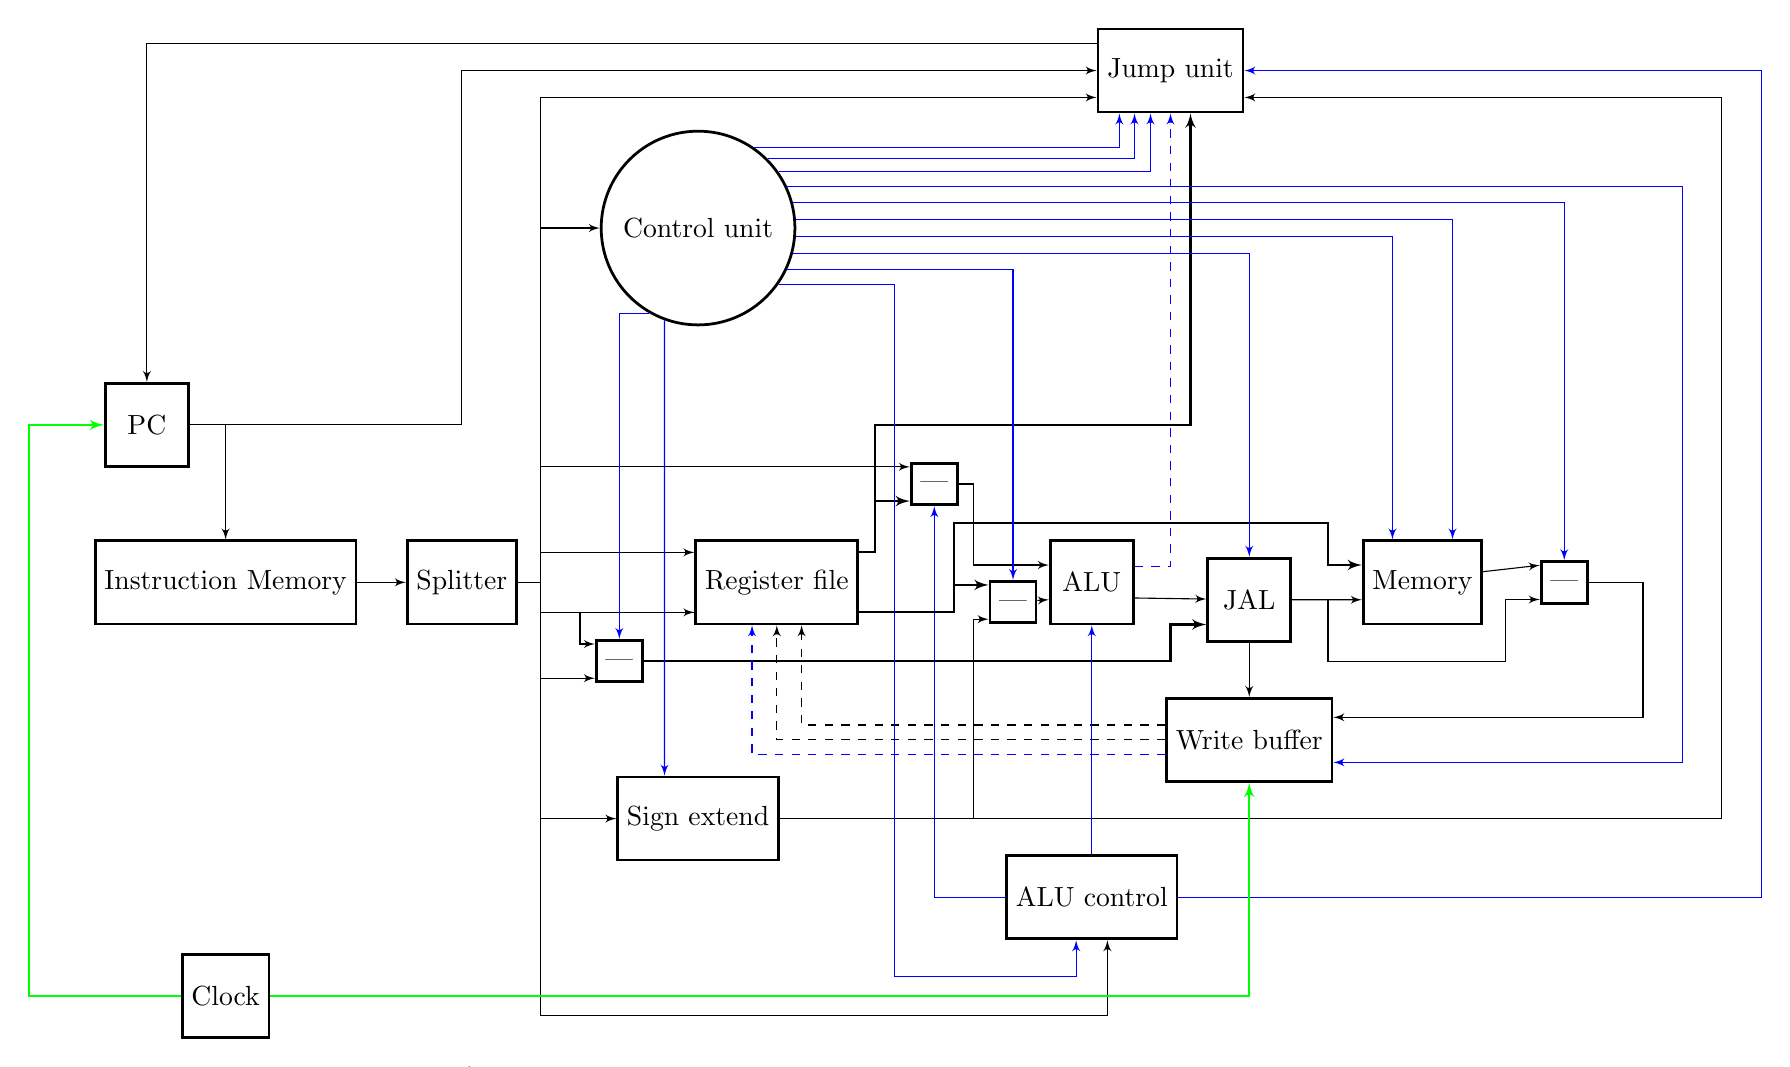
\begin{tikzpicture}
            \node[block] (reg) at (0,0) {Register file};
            \node[control] (cont) at (-1,4.5) {Control unit};
            \node[block] (jump) at (5,6.5) {Jump unit};
            \node[empty] (splitspace) at (-3,0) {};
            \node[block] (split) at (-4,0) {Splitter};
            \node[block] (if) at (-7,0) {Instruction Memory};
            \node[block] (sign) at (-1,-3) {Sign extend};
            \node[block] (alu) at (4,0) {ALU};
            \node[block] (alucont) at (4,-4) {ALU control};
            \node[block] (mem) at (8.2,0) {Memory};
            \node[block] (jal) at (6,-0.22) {JAL};
            \node[mux] (memread) at (10,0) {|};
            \node[mux] (shmt) at (2,1.25) {|};
            \node[mux] (imm) at (3, -0.25) {|};
            \node[mux] (regdst) at (-2,-1) {|};
            \node[block] (pc) at (-8, 2) {PC};
            \node[block] (writebuf) at (6, -2) {Write buffer};

            \path[draw, ->] (if) -- (split);
            \path[draw, -] (split) -- (splitspace.center);
            \path[draw, ->] (splitspace.center) |- (sign);
            \path[draw, ->] (splitspace.center) |- (cont);
            \path[draw, ->] (splitspace.center) |- (reg.160);
            \path[draw, ->] (splitspace.center) |- (reg.200);
            \path[draw, ->] (splitspace.center) |- (jump.200);
            \path[draw, ->] (splitspace.center) |- (2,-5.5) -| (alucont.290);
            \path[draw, ->] (splitspace.center) |- (regdst.215);
            \path[draw, ->] (splitspace.center) |- (shmt.145);
            \path[draw, ->] (reg.200) -| (-2.5, -0.5) |- (regdst.145);
            \path[draw, ->, color=blue] (alucont) -| (12.5, 0) |- (jump);
            \path[draw, ->, color=blue] (alucont) -| (shmt);
            \path[draw, thick, ->] (reg.340) -| (2.25,-0.25) |- (imm.145);
            \path[draw, thick, ->] (2.25,-0.25) |- (3,0.75) -- (7,0.75) |-
            (mem.164);
            \path[draw, thick, ->] (reg.20) -| (1.25,0.5) |- (shmt.215);
            \path[draw, thick, -] (1.25,0.5) |- (4,2);
            \path[draw, thick, ->] (4,2) -| (jump.295);
            \path[draw, ->] (shmt) -| (2.5, 0.5) |- (alu.158);
            \path[draw, ->, dashed, color=blue] (alu.20) -| (jump);
            \path[draw, ->] (alu.340) -- (jal);
            \path[draw, ->] (jal) -- (mem.196);
            \path[draw, ->] (imm) -- (alu.202);
            \path[draw, ->] (7, -0.22) |- (8, -1) -| (9.25,-0.5) |-
            (memread.215);
            \path[draw, ->] (mem.10) -- (memread.145);
            \path[draw, ->] (sign) -| (2.5, -1) |- (imm.215);
            \path[draw, ->] (2.5,-3) -| (12, 0) |- (jump.340);
            \path[draw, thick, ->] (regdst) -| (5, -0.6) |- (jal.210);
            \path[draw, ->] (pc) -| (if);
            \path[draw, ->] (pc) -| (-4, 4) |- (jump);
            \path[draw, ->] (jump.160) -| (pc);
            \path[draw, ->] (jal) -- (writebuf);
            \path[draw, ->] (memread) -| (11, -1) |- (writebuf.15);
            \path[draw, dashed, ->] (writebuf.170) -| (reg.300);
            \path[draw, dashed, ->] (writebuf) -| (reg);
            \path[draw, dashed, ->, color=blue] (writebuf.190) -| (reg.240);

            \path[draw, ->, color=blue] (alucont) -- (alu);
            \path[draw, ->, color=blue] (cont.55) -| (jump.220);
            \path[draw, ->, color=blue] (cont.45) -| (jump.230);
            \path[draw, ->, color=blue] (cont.35) -| (jump.245);
            \path[draw, ->, color=blue] (cont.25) -| (11.5,0) |-
            (writebuf.345);
            \path[draw, ->, color=blue] (cont.15) -| (memread);
            \path[draw, ->, color=blue] (cont.5) -| (mem.55);
            \path[draw, ->, color=blue] (cont.355) -| (mem.125);
            \path[draw, ->, color=blue] (cont.345) -| (jal);
            \path[draw, ->, color=blue] (cont.335) -| (imm);
            %\path[draw, ->, color=blue] (cont.325) -| (shmt);
            \path[draw, ->, color=blue] (cont.325) -| (1.5, -4) |-
            (2, -5) -| (alucont.250);
            \path[draw, ->, color=blue] (cont.250) -- (sign.128);
            \path[draw, ->, color=blue] (cont.240) -| (regdst);

            \node[block] (clock) at (-7, -5.25) {Clock};
            \path[draw, ->, thick, color=green] (clock) -| (-9.5,0) |- (pc);
            \path[draw, ->, thick, color=green] (clock) -| (writebuf);
        \end{tikzpicture}
    }
    \caption{Full single cycle MIPS processor. The units with | indicate
    multiplexors. Black wires indicate data wires. Blue wires indicate control
    wires. Green wires indicate clock}
    \label{fig:single-proc-full}
\end{figure}
% TODO hertil!
\subsection{Larger MIPS programs}
To test the full single cycle MIPS processor, we are going to implement two
programs in MIPS assembly: Quicksort and Towers Of Hanoi. We choose these two
examples, as both are simple to implement, and they do not require anything
special from the environment.

We are not going to give the implementation in MIPS assembly, as this would not
be readable. Instead, we are going to construct some low level \texttt{C} code,
which should be easy translatable into MIPS assembly. Once we have made the
assembly, we can easily dump it into MARS, which can then produce a ascii hex
dump, which we can then paste into our instruction memory.

\subsubsection*{Quicksort}
There are three parts of the Quicksort program: Loading data into memory,
the partition function and the quicksort function. We are going to use the
simple partition function from the algorithm book\cite{ref:alg}, and the
quicksort function, also from the algorithm book.

We could have implemented the Hoare partitioning algorithm. However, we are
trying to keep the program itself as simple as possible, as performance is not
the target of the program, but rather correctness of the processor, i.e.  that
our processor implementation produce the same result as MARS.

\begin{description}
    \item[Loading data into memory] We start by loading data into memory, so
        that our quicksort program has some data to sort. Which numbers we are
        going to use is not important, rather the amount of numbers, as the
        quicksort algorithm uses it as argument. We construct a function
        called \texttt{load()}, which inserts 6 numbers into the given memory
        address.
        \begin{lstlisting}
 void load(int *a) {
    *(a)   = 5;
    *(a+1) = 8;
    *(a+2) = 2;
    *(a+3) = 9;
    *(a+4) = 1;
    *(a+5) = 3;
}\end{lstlisting}

    \item[The partitioning function] Then we implement the \texttt{partition()}
        function as described in the algorithm book\cite{ref:alg}. Note that
        statements in the book have been expanded to more closely resemble
        assembly.
\begin{lstlisting}
int partition(int *a, int p, int r) {
    int x, i, j, tmp1, tmp2, *addr1, *addr2;
    addr1 = a + r;
    x = *(addr1);
    i = p - 1;
    for (j = p; j < r; j++) {
        addr1 = a + j;
        if (*(addr1) <= x) {
            i++;
            addr1 = a + i;
            addr2 = a + j;
            tmp1 = *(addr1);
            tmp2 = *(addr2);
            *(addr1) = tmp2;
            *(addr2) = tmp1;
        }
    }
    addr1 = a + i + 1;
    addr2 = a + r;
    tmp1 = *(addr1);
    tmp2 = *(addr2);
    *(addr1) = tmp2;
    *(addr2) = tmp1;
    return i + 1;
}
\end{lstlisting}

    \item[The quicksort function] Finally, we implement the
        \texttt{quicksort()} function as described in the algorithms book.
\begin{lstlisting}
void quicksort(int *a, int p, int r) {
    if (p < r) {
        int q = partition(a, p, r);
        quicksort(a, p, q-1);
        quicksort(a, q+1, r);
    }
}
\end{lstlisting}

    \item[Initial call to the algorithm] Bla bla main function
\begin{lstlisting}
main()
\end{lstlisting}
\end{description}
Do note that the arguments to both the \texttt{quicksort()} and
\texttt{partition()} functions, are inclusive. To verify the correctness, we
should look at the memory, where the initial data now should be in sorted
order.

\subsubsection*{Towers Of Hanoi}
Towers Of Hanoi is a puzzle, where one has to move a tower of discs, from one
peg, to another, with one additional auxilary peg, by only moving one disk at
the time.

Usually when searching for Towers Of Hanoi implementations, the program just
prints which move to make. However, since our processor does not support
printing at this state, we modify it. We are going to represent the three pegs
as an array, which is three times the size of the tower. As such, each peg is
just one third of the array.

\begin{description}
    \item[Loading data into memory] We need to initialize the memory. We are
        just going to fill the first third of the array with descending
        numbers.
\begin{lstlisting}
void init(int num, int *from, int *to, int *aux) {
    int i;
    for (i = 0; i < num; i++) {
        *(from+i) = num - i;
        *(to+i) = 0;
        *(aux+i) = 0;
    }
}
\end{lstlisting}

    \item[The tower function] This is the \texttt{tower()} function, which
        moves the disks from peg to peg.
\begin{lstlisting}
void tower(int num, int **from, int **to, int **aux) {
    int *t, *f;
    if (num == 1) {
        t = *to;
        f = *from;
        f--;
        *t = *f;
        t++;
        *f = 0;
        *to = t;
        *from = f;
    } else {
        tower(num-1, from, aux, to);
        t = *to;
        f = *from;
        f--;
        *t = *f;
        t++;
        *f = 0;
        *to = t;
        *from = f;
        tower(num-1, aux, to, from);
    }
}
\end{lstlisting}

    \item[Calling the algorithm] We construct a \texttt{main()} function, to
        ensure that the algorithm is correct, and that it can be run in regular
        \texttt{C}.
\begin{lstlisting}
int main() {
    int num = 5;
    int *arr = int[num*3];
    init(num, arr, arr+num, arr+(2*num));
}
\end{lstlisting}
\end{description}
When the program has finished, the last third of the array should contain the
numbers in descending order.


%\newpage
\section{Pipelining}
\label{sec:pipelining}
In this section, I will be looking at pipelining the single cycle MIPS
processor, and handle the problems, which are introduced by pipelining. I
start by going through the background and motivation for pipelining, and then
proceed on how to extend the single cycle MIPS processor to have pipes.

As mentioned, pipelining introduces new problems to handle in the processor,
and I will solve it by adding two new components: the Forwarding Unit, which
forwards results from previous instructions to later instructions, and the
Hazard Detection Unit, which controls when to stall the pipeline. Throughout
each step, I will also be writing programs, in order to verify that the
processor behaves as specified. The source code for the pipelined processor
with forwarding and hazard detection is available at~\cite{ref:github} in
\texttt{sme/src/Examples/PipelinedMIPS/}.

\subsection{Introducing the pipes}\label{sec:intro-pipe}
I have the single cycle MIPS processor, which accepts some of the core integer
instruction set. However, it is not very efficient, as the clock rate of the
processor is determined by the longest possible path in the processor. A path
in a processor is the components that a signal goes through, until it reaches a
safe state. A safe state in a processor is a state, where the signals are safely
stored in either registers or memory. A longer path implies a lower clockrate.
So in order to increase the clock rate, I must decrease the longest path in the
processor. I solve this by introducing pipes.

Pipes are registers in the processor, where all the values computed so far are
temporarely stored. It takes all of its inputs, and holds them until the next
clock tick, where it will forward the values it is holding. This ensures that
the data does not have to travel as far, until it have reached a safe state.

In order to know where to put the pipes, I divide the processor into stages.  I
will use the same stages, as proposed in the architecture book~\cite{ref:ark},
i.e. divide the processor into 5 stages: Instruction Fetch (IF), Instruction
Decode (ID), Execution (EX), Memory (MEM) and Write Back (WB). A simplified
overview of the processor and its stages can be seen in Figure~\ref{fig:stages}.
In between each stage, I am going to insert a pipe, i.e. I am
going to insert 4 pipes. The simplified processor with pipes can be seen in
Figure~\ref{fig:pipes}.

Introducing pipes also introduces additional problems, which I will discuss
further in sections~\ref{sec:forw} and~\ref{sec:haz}

\begin{figure}
    \centering
    \scalebox{0.5}{
        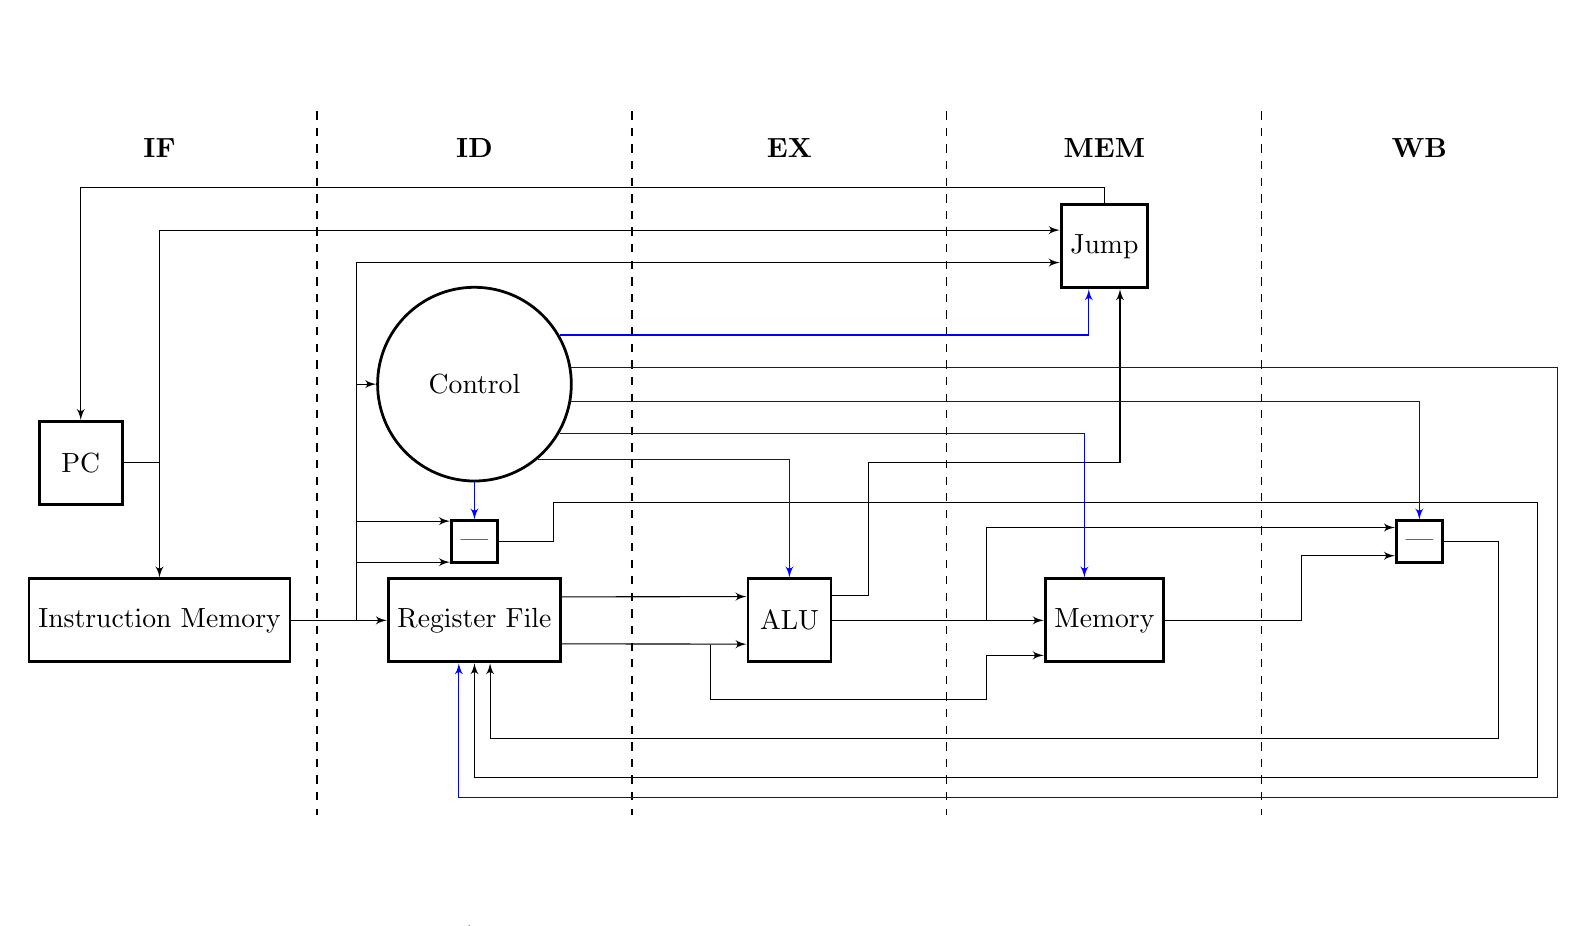
\begin{tikzpicture}
            \node[block] (alu) at (0,0) {ALU};
            \node[block] (reg) at (-4,0) {Register File};
            \node[block] (memo) at (4,0) {Memory};
            \node[block] (jump) at (4,4.75) {Jump};
            \node[block] (imem) at (-8,0) {Instruction Memory};
            \node[block] (pc) at (-9, 2) {PC};
            \node[control] (cont) at (-4, 3) {Control};
            \node[mux] (wbm) at (8,1) {|};
            \node[mux] (addr) at (-4, 1) {|};

            \node[empty] (if) at (-8, 6) {\textbf{IF}};
            \node[empty] (id) at (-4, 6) {\textbf{ID}};
            \node[empty] (ex) at (0, 6) {\textbf{EX}};
            \node[empty] (mem) at (4, 6) {\textbf{MEM}};
            \node[empty] (wb) at (8, 6) {\textbf{WB}};

            \node[empty] (ifidt) at (-6,7) {};
            \node[empty] (idext) at (-2,7) {};
            \node[empty] (exmemt) at (2,7) {};
            \node[empty] (memwbt) at (6,7) {};
            \node[empty] (ifidb) at (-6,-3) {};
            \node[empty] (idexb) at (-2,-3) {};
            \node[empty] (exmemb) at (2,-3) {};
            \node[empty] (memwbb) at (6,-3) {};

            \path[draw, dashed, -] (ifidt) -- (ifidb);
            \path[draw, dashed, -] (idext) -- (idexb);
            \path[draw, dashed, -] (exmemt) -- (exmemb);
            \path[draw, dashed, -] (memwbt) -- (memwbb);

            \path[draw, ->] (-5.5,0) |- (addr.220);
            \path[draw, ->] (-5.5,0) |- (addr.140);
            \path[draw, ->] (pc) -| (imem);
            \path[draw, ->] (imem) -- (reg);
            \path[draw, ->] (-5.5,0) |- (cont);
            \path[draw, ->] (reg.15) -- (alu.151);
            \path[draw, ->] (reg.345) -- (alu.209);
            \path[draw, ->] (alu) -- (memo);
            \path[draw, ->] (-1,-0.31) -| (-1,-1) -- (2.5,-1) |- (memo.210);
            \path[draw, ->] (2.5, 0) |- (wbm.150);
            \path[draw, ->] (memo) -- (6.5, 0) |- (wbm.210);
            \path[draw, ->] (wbm) -| (9, -1.5) -| (reg.290);
            \path[draw, ->] (alu.30) -| (1,1) |- (4,2) -| (jump.290);
            \path[draw, ->] (jump) |- (0,5.5) -| (pc);
            \path[draw, ->] (-8,2) |- (jump.160);
            \path[draw, ->] (-5.5,3) |- (jump.200);
            \path[draw, ->] (addr) -| (-3, 1.5) -| (9.5,-2) -|
            (reg.270);

            %\path[draw, color=blue, ->] (cont) -- (reg);
            %\path[draw, color=blue, ->] (cont.10) -| (9.5,-2) -| (reg.250);
            \path[draw, color=blue, ->] (cont.10) -| (9.75,-2.25) -| (reg.250);
            \path[draw, color=blue, ->] (cont.310) -| (alu);
            \path[draw, color=blue, ->] (cont.330) -| (memo.115);
            \path[draw, color=blue, ->] (cont.350) -| (wbm);
            \path[draw, color=blue, ->] (cont.30) -| (jump.250);
            \path[draw, color=blue, ->] (cont) -- (addr);
        \end{tikzpicture}
    }
    \caption{The simplified single cycle processor, and its stages. The stage
    names are highlighted in \textbf{bold}. The stages are divided by dashed
    lines.}
    \label{fig:stages}
\end{figure}
\begin{figure}
    \centering
    \scalebox{0.5}{
        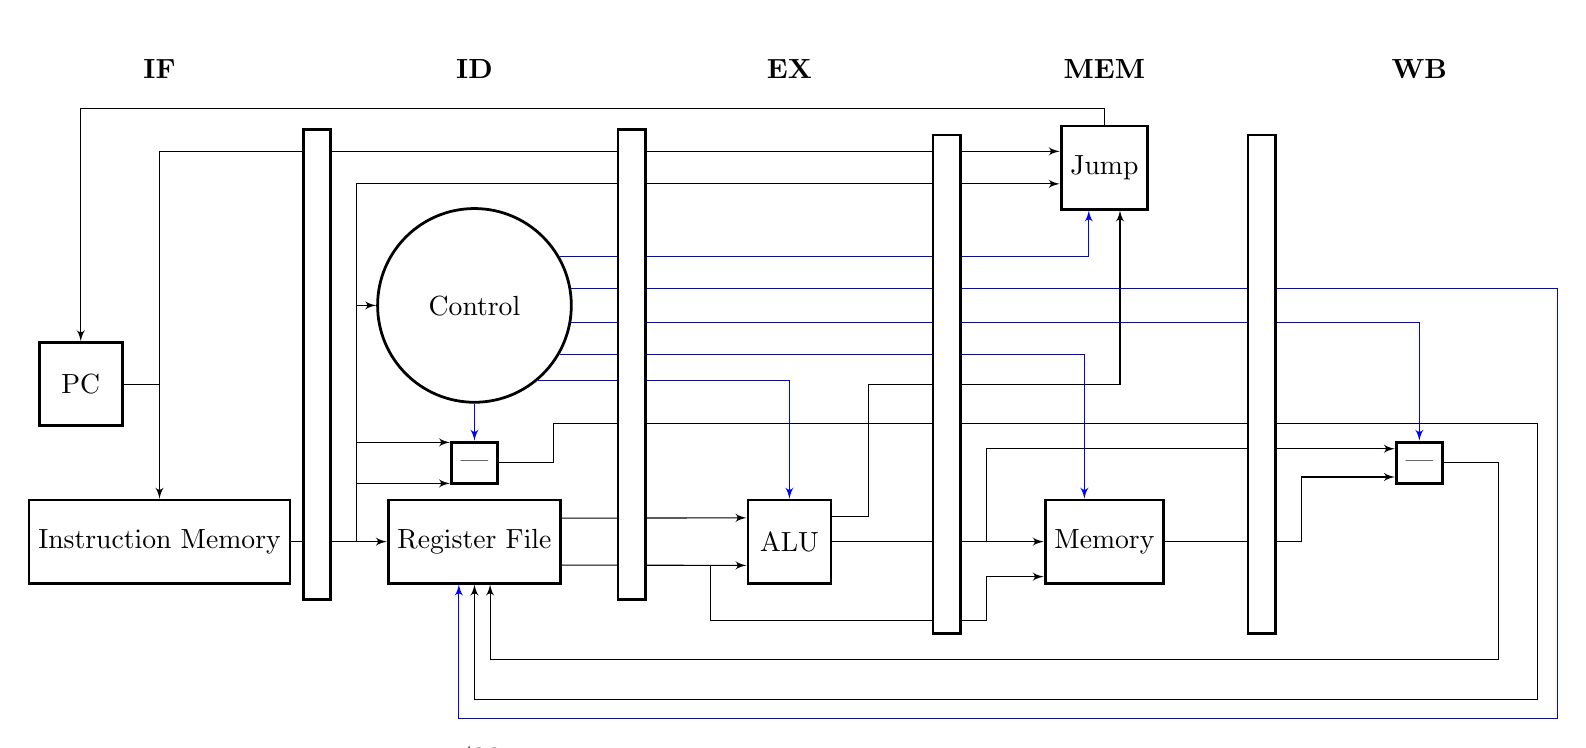
\begin{tikzpicture}
            \node[block] (alu) at (0,0) {ALU};
            \node[block] (reg) at (-4,0) {Register File};
            \node[block] (memo) at (4,0) {Memory};
            \node[block] (jump) at (4,4.75) {Jump};
            \node[block] (imem) at (-8,0) {Instruction Memory};
            \node[block] (pc) at (-9, 2) {PC};
            \node[control] (cont) at (-4, 3) {Control};
            \node[mux] (wbm) at (8,1) {|};
            \node[mux] (addr) at (-4, 1) {|};

            \node[empty] (if) at (-8, 6) {\textbf{IF}};
            \node[empty] (id) at (-4, 6) {\textbf{ID}};
            \node[empty] (ex) at (0, 6) {\textbf{EX}};
            \node[empty] (mem) at (4, 6) {\textbf{MEM}};
            \node[empty] (wb) at (8, 6) {\textbf{WB}};

            \path[draw, ->] (-5.5,0) |- (addr.220);
            \path[draw, ->] (-5.5,0) |- (addr.140);
            \path[draw, ->] (pc) -| (imem);
            \path[draw, ->] (imem) -- (reg);
            \path[draw, ->] (-5.5,0) |- (cont);
            \path[draw, ->] (reg.15) -- (alu.151);
            \path[draw, ->] (reg.345) -- (alu.209);
            \path[draw, ->] (alu) -- (memo);
            \path[draw, ->] (-1,-0.31) -| (-1,-1) -- (2.5,-1) |- (memo.210);
            \path[draw, ->] (2.5, 0) |- (wbm.150);
            \path[draw, ->] (memo) -- (6.5, 0) |- (wbm.210);
            \path[draw, ->] (wbm) -| (9, -1.5) -| (reg.290);
            \path[draw, ->] (alu.30) -| (1,1) |- (4,2) -| (jump.290);
            \path[draw, ->] (jump) |- (0,5.5) -| (pc);
            \path[draw, ->] (-8,2) |- (jump.160);
            \path[draw, ->] (-5.5,3) |- (jump.200);
            \path[draw, ->] (addr) -| (-3, 1.5) -| (9.5,-2) -|
            (reg.270);

            \path[draw, color=blue, ->] (cont.310) -| (alu);
            \path[draw, color=blue, ->] (cont.330) -| (memo.115);
            \path[draw, color=blue, ->] (cont.350) -| (wbm);
            %\path[draw, color=blue, ->] (cont.10) -| (9.5,-2) -| (reg.250);
            \path[draw, color=blue, ->] (cont.10) -| (9.75,-2.25) -| (reg.250);
            \path[draw, color=blue, ->] (cont.30) -| (jump.250);
            \path[draw, color=blue, ->] (cont) -- (addr);

            \node[block, minimum height=170, minimum width=10, fill=white] (ifid) at
            (-6,2.25) {};
            \node[block, minimum height=170, minimum width=10, fill=white] (idex) at
            (-2,2.25) {};
            \node[block, minimum height=180, minimum width=10, fill=white]
            (exmem) at (2,2) {};
            \node[block, minimum height=180, minimum width=10, fill=white]
            (exmem) at (6,2) {};
        \end{tikzpicture}
    }
    \caption{The simplified pipelined processor. The long bars in between each
    state are the pipes.}
    \label{fig:pipes}
\end{figure}

\subsubsection*{Implementation}
There are two ways to implement pipes in SME: by using clocked busses, or by
using clocked processes. If the bus only traverses two stages, then I can use
clocked busses, as the semantics of a clocked bus is exactly the same as a
pipe (i.e. the value is not passed along the bus, until the clock ticks).
However, if the bus traverses more than two stages, I am going to need
additional processes, as the clocked bus only stores its value for one clock
tick. Furthermore, if the only change to the bus is the given
\texttt{ClockedBus} attribute, then determining whether or not a bus is part of
a pipe can be problematic. As such, I have the pipe and its busses in their own
class, as it then receives its own namespace, and the code then becomes more
readable.

Let us take a subset of the IF/ID pipe, as an example. I assume that each
state is in its own classes, i.e. \texttt{IF} and \texttt{ID}, and that the
\texttt{IF} stage has the \texttt{Instruction} bus, which the \texttt{ID} stage
reads from. Then, by adding a subclass to the \texttt{IF} stage, the name of
the bus that the \texttt{ID} class calls is converteted from
\texttt{IF.Instruction} to \texttt{IF.Pipe.Instruction}, emphasizing that the
value is now fetched from the piped bus.

Introducing the pipes in this manner is fairly straightforward, as I just
add 4 classes, each with the same set of busses as the 'previous' stage outputs
to the 'next' stage, and each with a register process, which forwards all the
values from the 'previous' stages busses, onto its own busses with the same
name.

This process can be repeated for all of the required pipes. By following the
division of the components, as proposed in the architecture book~\cite{ref:ark},
there is only one really tricky part of pipelining: the Jump Unit. The
processor does not know whether to jump until the \texttt{MEM} stage, as the
computations are made in the \texttt{EX} stage, and the conditions are computed
in the \texttt{MEM} stage. However, the Program Counter has to increment,
regardless of whether or not it should jump. As such, I should divide the Jump
Unit into its subcomponents, and place some of the logic in the \texttt{IF},
some in the \texttt{EX} stage and finally some of it in the \texttt{MEM} stage.

For the \texttt{IF} stage, the incrementer and a multiplexor should be placed
inside the stage. The multiplexor should take an address computed from the
\texttt{MEM} stage, and the incremented Program Counter, and based on whether
or not the instruction that has reached the \texttt{MEM} stage was a branch or
jump instruction, it should choose the computed address.

The core computation of the jump and branch instructions should be placed in
the \texttt{EX} stage. As such, the \texttt{EX} stage should compute both the
branch address and the jump address.

Finally, the \texttt{MEM} stage should hold the decision logic. First, it
should determine if the instruction was an branch instruction, and whether or
not the condition has been satisfied, in which case, the address forwarded to
the \texttt{IF} stage should be the branch address. If this was not the case,
the computed jump address should be the one forwarded.

Finally, in the single cycle MIPS processor, I introduced the Write Buffer, in
order to remove the cycle from and to the Register File. However, by
introducing pipes, I have introduced a new buffer, and thus the Write Buffer
can be removed.

\subsubsection*{Testing}
To test the processor, I can use any of the programs, that I have previously
written. However, since I have pipelined the processor, I need to insert
bubbles, in order for data to be available for each instruction. A bubble is a
No Operation (\texttt{nop}) instruction, which performs no operation, and does
not modify neither the Register File nor the Memory.

I am going to implement a simple program, which is easy to verify: a small
loop, which computes $n$ fibonacci numbers, and places them in memory. As with
the simple cycle, I am going to give pseudo low level C code:
\begin{lstlisting}
void init(int *arr) {
    *(arr)   = 1;
    *(arr+1) = 1;
}

void loop(int *arr, int n) {
    int i, tmp1, tmp2, tmp3;
    for (i = 0; i < n; i++) {
        tmp1 = *(arr+i);
        tmp2 = *(arr+i+1);
        tmp3 = tmp1 + tmp2;
        *(arr+i+2) = tmp3;
    }
}
\end{lstlisting}
Note that for verification in C, the size of the array should be $n+2$, due to
initialization. Furthermore, when I port it to MIPS assembly, after each
instruction, I insert four \texttt{nop}'s, to ensure the data is ready for the
next instruction. When the program has run, the $n+2$ fibonacci numbers should
be in memory, at the given address.

\subsection{Forwarding}\label{sec:forw}
By introducing pipes, I also introduced data hazards and control hazards. I
will go through control hazards in Section~\ref{sec:haz}. Data hazards are when
one instruction writes to a register, that a following instruction reads from.
This is not a problem in the single cycle processor, as all data have been
written to registers in the same clock cycle. This is not the case in the
pipelined processor, e.g. the data might reside in the MEM stage, when it is
needed in the EX stage.

I can eliminate some of the data hazards by implementing an additional unit:
the Forwarding Unit. The rest of the data hazards will be handled by hazard
detection in Section~\ref{sec:haz}. The Forwarding Unit looks at the register
addresses used by the instruction in the EX stage, and checks if it corresponds
with the register write address of either the instruction in the MEM stage, or
the instruction in the WB stage. If they correspond, it forwards the value from
either the MEM or the WB stage to the EX stage. The overview of the simplified
processor with the forwarding unit can be seen in Figure~\ref{fig:forw}.

I could also have gone with the bubble approach, i.e. insert bubbles every
time there is a data hazard. However, this would not be optimal, as this would
result in several clock ticks, where the processor is idle.

\begin{figure}
    \centering
    \scalebox{0.5}{
        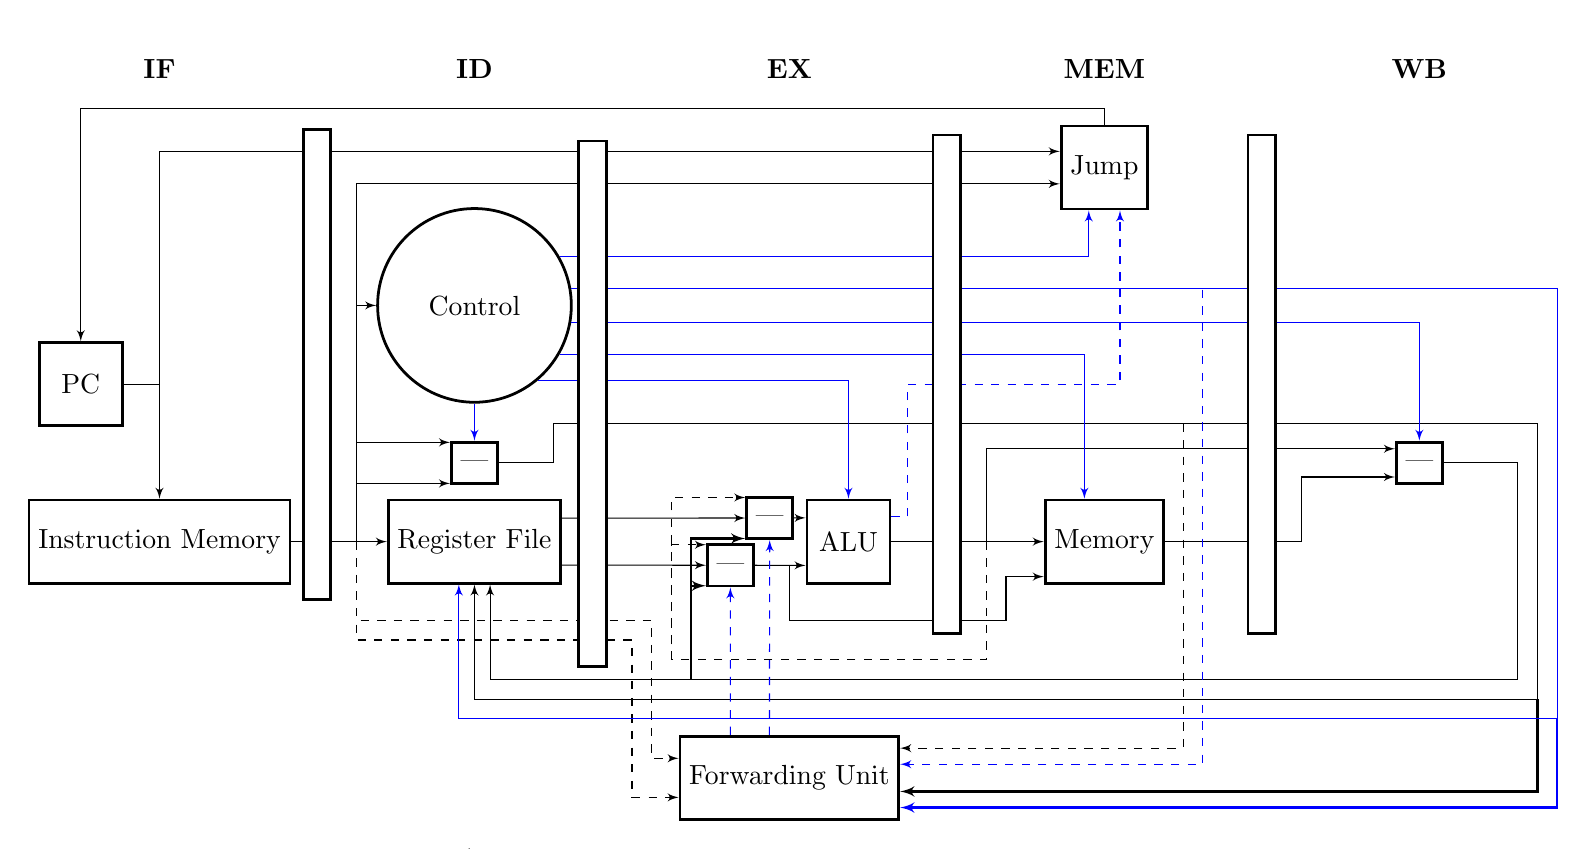
\begin{tikzpicture}
            \node[block] (alu) at (0.75,0) {ALU};
            \node[block] (reg) at (-4,0) {Register File};
            \node[block] (memo) at (4,0) {Memory};
            \node[block] (jump) at (4,4.75) {Jump};
            \node[block] (imem) at (-8,0) {Instruction Memory};
            \node[block] (pc) at (-9, 2) {PC};
            \node[control] (cont) at (-4, 3) {Control};
            \node[mux] (wbm) at (8,1) {|};
            \node[block] (forw) at (0, -3) {Forwarding Unit};
            \node[mux] (forwa) at (-0.25, 0.3) {|};
            \node[mux] (forwb) at (-0.75, -0.3) {|};
            \node[mux] (addr) at (-4, 1) {|};

            \node[empty] (if) at (-8, 6) {\textbf{IF}};
            \node[empty] (id) at (-4, 6) {\textbf{ID}};
            \node[empty] (ex) at (0, 6) {\textbf{EX}};
            \node[empty] (mem) at (4, 6) {\textbf{MEM}};
            \node[empty] (wb) at (8, 6) {\textbf{WB}};

            \path[draw, ->] (pc) -| (imem);
            \path[draw, ->] (imem) -- (reg);
            \path[draw, ->] (-5.5,0) |- (cont);
            \path[draw, ->] (-5.5,0) |- (addr.220);
            \path[draw, ->] (-5.5,0) |- (addr.140);
            %\path[draw, ->] (reg.15) -- (alu.151);
            \path[draw, ->] (reg.15) -- (forwa);
            \path[draw, ->] (forwa) --  (alu.151);
            \path[draw, ->] (reg.345) -- (forwb);
            \path[draw, ->] (forwb) -- (alu.209);
            \path[draw, ->] (alu) -- (memo);
            \path[draw, ->] (0,-0.3) |- (0,-1) -- (2.75,-1) |- (memo.210);
            \path[draw, ->] (2.5, 0) |- (wbm.150);
            \path[draw, ->] (memo) -- (6.5, 0) |- (wbm.210);
            \path[draw, ->] (wbm) -| (9.25, -1.75) -| (reg.290);
            \path[draw, color=blue, dashed, ->] (alu.30) -| (1.5,1) |- (4,2) -| (jump.290);
            \path[draw, ->] (jump) |- (0,5.5) -| (pc);
            \path[draw, ->] (-8,2) |- (jump.160);
            \path[draw, ->] (-5.5,3) |- (jump.200);
            \path[draw, thick, ->] (-1.25,-1.75) |- (forwb.220);
            \path[draw, thick, ->] (-1.25,-1.75) |- (forwa.220);
            \path[draw, dashed, ->] (2.5, 0) |- (-1.5, -1.5) |- (forwb.140);
            \path[draw, dashed, ->] (-1.5, -1.5) |- (forwa.140);
            \path[draw, ->] (addr) -| (-3, 1.5) -| (9.5,-2) -|
            (reg.270);
            \path[draw, thick, ->] (9.5, -2) |- (forw.353);
            \path[draw, dashed, ->] (5,1.5) |- (forw.15);
            \path[draw, dashed, ->] (-5.5,0) |- (-1.75,-1) |- (forw.170);
            \path[draw, dashed, ->] (-5.5,0) |- (-2,-1.25) |- (forw.190);

            \path[draw, color=blue, ->] (cont.310) -| (alu);
            \path[draw, color=blue, ->] (cont.330) -| (memo.115);
            \path[draw, color=blue, ->] (cont.350) -| (wbm);
            \path[draw, color=blue, ->] (cont.10) -| (9.75,-2.25) -| (reg.250);
            \path[draw, color=blue, ->] (cont.30) -| (jump.250);
            \path[draw, color=blue, ->] (cont) -- (addr);
            \path[draw, color=blue, thick, ->] (9.75,-2.25) |- (forw.345);
            \path[draw, color=blue, dashed, ->] (5.25, 3.2) |- (forw.7);

            \path[draw, color=blue, dashed, ->] (forw.115) -- (forwa);
            \path[draw, color=blue, dashed, ->] (forw.144) -- (forwb);


            \node[block, minimum height=170, minimum width=10, fill=white] (ifid) at
            (-6,2.25) {};
            \node[block, minimum height=190, minimum width=10, fill=white] (idex) at
            (-2.5,1.75) {};
            \node[block, minimum height=180, minimum width=10, fill=white]
            (exmem) at (2,2) {};
            \node[block, minimum height=180, minimum width=10, fill=white]
            (exmem) at (6,2) {};
        \end{tikzpicture}
    }
    \caption{The simplified pipelined processor with forwarding.}
    \label{fig:forw}
\end{figure}

\subsubsection*{Implementation}
Implementing the Forwarding Unit should be done with an SME process. As it
interferes with the EX stage, it should be put in the EX stage. The unit should
be controlling two multiplexors. The first multiplexor should control whether
Output A should come from the ID pipe, the write data from the MEM stage or the
write data from the WB stage. The other multiplexor is analogous, but with
Output B. The two multiplexors should be controlled by the Forwarding Unit,
i.e. it should generate the control signals for the multiplexors based on the
two register read addresses of the current instruction in the EX stage, the
register write address and write enabled signal both from the MEM and the WB
stages.

\subsubsection*{Testing}
Testing is straightforward: I can just remove all of the \texttt{nop}'s from
the fibonacci program, except for those which come after either a load, a
branch or a jump, as these hazards are not handled yet.

\subsection{Hazard Detection}\label{sec:haz}
As mentioned in Section~\ref{sec:forw}, I cannot avoid all data hazards with
forwarding. This is because it only forwards to the EX stage. However,
if the instruction prior to the instruction in EX is a load, then the data wont
be available, until the load instruction has reached the WB stage. To handle
this, the processor needs to detect the hazard and insert a bubble, as this
will delay the instruction, so that when it has reached the EX stage, the load
instruction will be in the WB stage, and thus it can be forwarded. When
inserting a bubble in the middle of the pipeline, some of the pipes and
registers must also be stalled. Stalling is the action of outputting what is stored
in the register, but not updating it, i.e. outputting the same data in the
next clock tick.

I also need to be able to handle an additional type of hazard: control
hazards. Control hazards are when either jump or branch instructions are
executed. The problem is that the branch or jump is not performed until the MEM
stage, which means that the pipeline following the jump or branch instruction
may have been filled up by instructions, which should not be executed. To solve
this, it should detect the hazard, and in such case flush the pipeline.
Flushing the pipeline, is the action of resetting the registers in the pipes,
so that they output a \texttt{nop} instruction. The overview of the simplified
processor with the Hazard Detection Unit can be seen in Figure~\ref{fig:hazard}.

\begin{figure}
    \centering
    \scalebox{0.5}{
        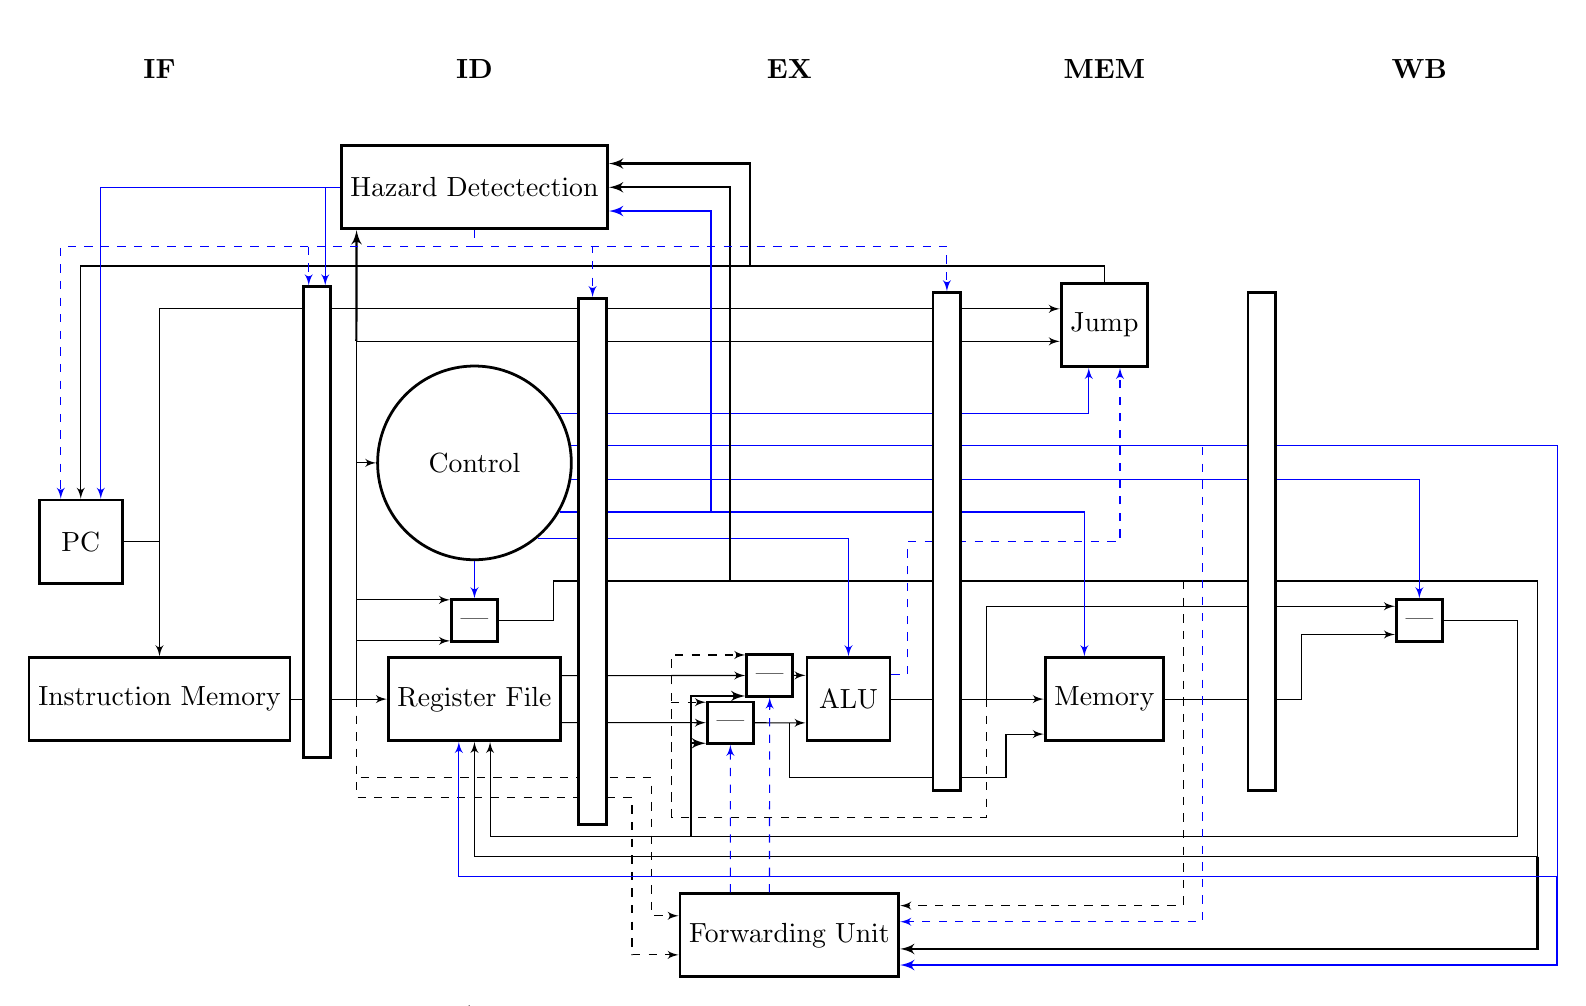
\begin{tikzpicture}
            \node[block] (alu) at (0.75,0) {ALU};
            \node[block] (reg) at (-4,0) {Register File};
            \node[block] (memo) at (4,0) {Memory};
            \node[block] (jump) at (4,4.75) {Jump};
            \node[block] (imem) at (-8,0) {Instruction Memory};
            \node[block] (pc) at (-9, 2) {PC};
            \node[control] (cont) at (-4, 3) {Control};
            \node[mux] (wbm) at (8,1) {|};
            \node[block] (forw) at (0, -3) {Forwarding Unit};
            \node[mux] (forwa) at (-0.25, 0.3) {|};
            \node[mux] (forwb) at (-0.75, -0.3) {|};
            \node[mux] (addr) at (-4, 1) {|};
            \node[block] (haz) at (-4,6.5) {Hazard Detectection};

            \node[empty] (if) at (-8, 8) {\textbf{IF}};
            \node[empty] (id) at (-4, 8) {\textbf{ID}};
            \node[empty] (ex) at (0, 8) {\textbf{EX}};
            \node[empty] (mem) at (4, 8) {\textbf{MEM}};
            \node[empty] (wb) at (8, 8) {\textbf{WB}};

            \path[draw, ->] (pc) -| (imem);
            \path[draw, ->] (imem) -- (reg);
            \path[draw, ->] (-5.5,0) |- (cont);
            \path[draw, ->] (-5.5,0) |- (addr.220);
            \path[draw, ->] (-5.5,0) |- (addr.140);
            %\path[draw, ->] (reg.15) -- (alu.151);
            \path[draw, ->] (reg.15) -- (forwa);
            \path[draw, ->] (forwa) --  (alu.151);
            \path[draw, ->] (reg.345) -- (forwb);
            \path[draw, ->] (forwb) -- (alu.209);
            \path[draw, ->] (alu) -- (memo);
            \path[draw, ->] (0,-0.3) |- (0,-1) -- (2.75,-1) |- (memo.210);
            \path[draw, ->] (2.5, 0) |- (wbm.150);
            \path[draw, ->] (memo) -- (6.5, 0) |- (wbm.210);
            \path[draw, ->] (wbm) -| (9.25, -1.75) -| (reg.290);
            \path[draw, color=blue, dashed, ->] (alu.30) -| (1.5,1) |- (4,2) -| (jump.290);
            \path[draw, ->] (jump) |- (0,5.5) -| (pc);
            \path[draw, ->] (-8,2) |- (jump.160);
            \path[draw, ->] (-5.5,3) |- (jump.200);
            \path[draw, thick, ->] (-1.25,-1.75) |- (forwb.220);
            \path[draw, thick, ->] (-1.25,-1.75) |- (forwa.220);
            \path[draw, dashed, ->] (2.5, 0) |- (-1.5, -1.5) |- (forwb.140);
            \path[draw, dashed, ->] (-1.5, -1.5) |- (forwa.140);
            \path[draw, ->] (addr) -| (-3, 1.5) -| (9.5,-2) -|
            (reg.270);
            \path[draw, thick, ->] (9.5, -2) |- (forw.353);
            \path[draw, dashed, ->] (5,1.5) |- (forw.15);
            \path[draw, dashed, ->] (-5.5,0) |- (-1.75,-1) |- (forw.170);
            \path[draw, dashed, ->] (-5.5,0) |- (-2,-1.25) |- (forw.190);

            \path[draw, color=blue, ->] (cont.310) -| (alu);
            \path[draw, color=blue, ->] (cont.330) -| (memo.115);
            \path[draw, color=blue, ->] (cont.350) -| (wbm);
            \path[draw, color=blue, ->] (cont.10) -| (9.75,-2.25) -| (reg.250);
            \path[draw, color=blue, ->] (cont.30) -| (jump.250);
            \path[draw, color=blue, ->] (cont) -- (addr);
            \path[draw, color=blue, thick, ->] (9.75,-2.25) |- (forw.345);
            \path[draw, color=blue, dashed, ->] (5.25, 3.2) |- (forw.7);

            \path[draw, color=blue, dashed, ->] (forw.115) -- (forwa);
            \path[draw, color=blue, dashed, ->] (forw.144) -- (forwb);

            % Hazard
            \path[draw, thick, ->] (-0.75, 1.5) |- (haz); % addr
            \path[draw, thick, color=blue, ->] (-1, 2.37) |- (haz.350); % mem
            \path[draw, thick, ->] (-0.5, 5.5) |- (haz.10); % pcsrc
            \path[draw, thick, ->] (-5.5, 4.55) -- (haz.200);% reada readb
            \path[draw, dashed, color=blue, -] (haz) -- (-4, 5.75);

            \node[block, minimum height=170, minimum width=10, fill=white] (ifid) at
            (-6,2.25) {};
            \node[block, minimum height=190, minimum width=10, fill=white] (idex) at
            (-2.5,1.75) {};
            \node[block, minimum height=180, minimum width=10, fill=white]
            (exmem) at (2,2) {};
            \node[block, minimum height=180, minimum width=10, fill=white]
            (memwb) at (6,2) {};

            \path[draw, dashed, color=blue, ->] (-4, 5.75) -| (exmem);
            \path[draw, dashed, color=blue, ->] (-4, 5.75) -| (idex);
            \path[draw, dashed, color=blue, ->] (-4, 5.75) -| (ifid.92);
            \path[draw, dashed, color=blue, ->] (-4, 5.75) -| (pc.115);
            \path[draw, color=blue, ->] (haz) -| (ifid.88);
            \path[draw, color=blue, ->] (haz) -| (pc.65);
        \end{tikzpicture}
    }
    \caption{The simplified pipelined processor with forwarding and hazard
    detection.}
    \label{fig:hazard}
\end{figure}

\subsubsection*{Implementation}
The hazard detection should be implemented in its own SME process: the Hazard
Detection Unit.

To solve the data hazards, it needs to read the \texttt{memread} control flag
from the EX stage, the register write address from the EX stage and the two
source register addresses from the ID stage. If the \texttt{memread} flag has
been set, and either of the source registers match the destination register,
then the ID/EX pipe should be flushed, the IF/ID pipe should be stalled, and
the PC register should be stalled.

To solve the control hazards, it should read the \texttt{PCSrc} flag from the
MEM stage (the one used by the PC register, to multiplex between the
incremented address, and the jump/branch address), and if it is set, then the
IF/ID, ID/EX and EX/MEM pipes should be flushed. Note: the PC register should
read normally in the case of a flush, even though it might have to stall, as
the stall is detected in the pipe that is being flushed.

\subsubsection*{Testing}
Testing the new hazard detection is straightforward, as the processor should
now be able to handle all of the previous programs, albeit in a larger amount
of clock ticks, compared to the single cycle processor. The performance of the
processor with hazard detection can be seen in Table~\ref{tab:perf-pipe}.

\begin{table}
    \centering
    \begin{adjustbox}{center}
    \begin{tabular}{rlllllllllll}
        & & \texttt{MARS} & & & \texttt{SME} \\
        \hline
        & & \# CT & time (ms) & CR (hz) &
            \# CT & time (ms) & CR (hz) \\
        \hline
        Towers of Hanoi & $n=5$ &
            719        & 585        & $\sim$1229 &
            720 - 1058 & 516 - 1190 & $\sim$1395 - $\sim$889 \\

        Quicksort & $n=8$ &
            483       & 852       & $\sim$829 &
            484 - 763 & 375 - 895 & $\sim$1290 - $\sim$852 \\

        Fib no optimization & $n=10$ &
            220       & 584       & $\sim$376 &
            221 - 251 & 191 - 356 & $\sim$1157 - $\sim$753 \\

        Fib forward & $n=10$ &
            98        & 586       & $\sim$167 &
            100 - 130 & 119 - 209 & $\sim$840 - $\sim$ 622 \\

        Fib hazard & $n=10$ &
            84       & 588       & $\sim$142 &
            86 - 126 & 113 - 212 & $\sim$761 - $\sim$594 \\
        \hline
    \end{tabular}
    \end{adjustbox}
    \caption{Performance of the Quicksort, Towers of Hanoi and different
    versions of the fibonacci programs. CT is clock ticks. CR is clockrate.
    In the columns with multiple values, the left value is the performance of
    the single cycle processor and the right is the performance of the pipelined
    processor. The benchmark was performed on a laptop with an Intel Core
    i5-5300U (2.3 GHz).}
    \label{tab:perf-pipe}
\end{table}


By looking at the performance in Table~\ref{tab:perf-pipe}, I see that the
performance of the pipelined processor is worse both in execution time, clock
ticks and clockrate. The additional clock ticks are expected of the pipelined
processor, as there is an wind-up time for filling the pipeline, and as I loose
some instructions by stalling and flushing.

By looking at the fibonacci program with hazard detection, I see that the
single cycle processor uses 86 clock ticks. It runs the loop 10 times and for
each branch it flushes the pipeline, i.e. losing $10 \times 3 = 30$
instructions. Furthermore, there is a dependency following a load instruction,
producing a stall in each loop, i.e. losing an additional 10 instructions. By
summing this up, I get $86 + 30 + 10 = 126$, which is exactly the
amount of instructions performed by the pipelined processor.

The execution time of the SME simulation, and as such also the simulation
clockrate, is worse. This is due to the SME simulation having more work to do,
as I have increased the amount of processes and busses. There should not be any
decrease in performance when synthesized to FPGA, but rather an increase.
As mentioned in Section~\ref{sec:intro-pipe}, it is because I should be able
to increase the clockrate, compared to the single cycle implementation.


%\newpage
\section{Transpiling and synthesizing SME}
\label{sec:synthesis}
In this section, I will be describing the steps required to implement an SME
network onto an actual FPGA. I start with the initial logic gates design, as it
is very simple to verify, and because it does not have any requirements
regarding clocking.

Then I will be implementing the single cycle MIPS processor, and finally show
how to communicate with the hardware implemented on the FPGA. This section will
be very hardware specific, as I have not had time to verify or develop an
approach, which will run on additional hardware.

\subsection{General workflow}
TODO figur! SME > ghdl > vivado func > vivado post-impl > bitstream > interface func >
export > SDK.

In order to implement hardware onto an FPGA, one must describe the hardware
using a hardware description language such as VHDL or Verilog. As mentioned
before, SME can be transpiled into VHDL, and as such provides a high level
approach for hardware design. Therefore, the first thing to do is to write an
SME network, verify that it runs as expected, and then checking that the
transpiler does not fail to transpile.

Once the VHDL has been generated, the VHDL can be verified by using
\texttt{ghdl}. \texttt{ghdl} is an commandline simulator for VHDL. SME provides
a testbench and a \texttt{Makefile} for running the testbench using
\texttt{ghdl}. As such, to verify the generated VHDL, one only needs to run
\texttt{make} inside the output \texttt{vhdl/} folder.

Processor is clocked at 5mhz!


\newpage
\section{Conclusion}
I have succesfully implemented a MIPS processor in the SME programming model,
in the timeframe of $\sim$2 months. This shows that the SME model is
suitable for designing hardware, with the prior knowledge of the CSP model,
hardware organization and software development.

Furthermore, by extending the accepted instruction set, and by pipelining the
processor, I have shown that extending the initial design in order to gain
increased performance or additional functionality, is possible.

I have also shown that SME indeed can be transpiled into functioning VHDL, with
a small amount of extra work. The extra actions are however simple enough, such
that they could be implemented in a future version of SME.

As such, with the material in this thesis, a computer science student, such as
myself, should be able to construct specialized hardware by using SME, in the
timeframe of a university course.

%As such, with the material in this paper, everyone with a computer science
%background should be able to construct specialized hardware by using SME.


%\newpage
\section{Future work}
The initial step would be to add an AXI interface to the Pipelined processor.
The approach is the same as with the single cycle processor. It would be
interesting to see whether or not the increased clock is applicable to the
additional AXI interface.
% The initial step would be to synthesize and implement the pipelined processor.
% Given that I have already stated the approach for the single cycle processor,
% this should not be too hard. It could be interesting to see, if it can be
% clocked higher and in that case how much. Furthermore, it would also be more
% usable, as it should have access to more memory.

Inspired by the manycore architecture of the SW26010 processors in the
TaihuLight supercomputer~\cite{ref:supercomputer}, I want to see how many
cores I am able to fit onto a single FPGA. By doing this, I also want to
introduce scratchpad memory, instead of focusing on the traditional memory
hierarchy, as this is what is being used in the SW26010.

It would also be interesting to extend the processor core, to a superscalar
processor, i.e. by introducing multiple execution paths. This could both be by
introducing additional ALUs, e.g. floating point, or by introducing
coprocessors, which are specialized for certain tasks, such as the SME network
of a student project, which solved partial differential equations and fast
fourier transforms.

A final suggestion would be to extend the processor with the required
components, such that a minimal operating system could be compiled and run on
the processor. This would be useful in specialized hardware, if a device should
run purely in its own environment.


\newpage
%\section{References}
%\begin{thebibliography}{9}
    \bibitem{ref:sme} Brian Vinter \& Kenneth Skovhede. \it{Synchronous Message
        Exchange for Hardware Designs}. \copyright\ The authors and Open
        Channel Publishing Ltd. 2014.
    \bibitem{ref:csp} C.A.R. Hoare. \it{Communicating Sequential Processes}.
        \copyright\ ACM 1978.
    \bibitem{ref:ark} David A. Patterson \& John L. Hennessy. \it{Computer
        Organization and Design - The Hardware/Software Interface (Revised 4th
        edition)}.  \copyright\ Elsevier 2012.
    \bibitem{ref:diku} \it{Maskinarkitektur (ARK) 2013/2014}
        \url{http://kurser.ku.dk/course/ndaa04009u/2013-2014}
    \bibitem{ref:logic} Introduction to Combinational Logic Functions
        \url{https://www.allaboutcircuits.com/textbook/digital/chpt-9/combinational-logic-functions/}
    \bibitem{ref:alg} Thomas H. Cormen, Charles E. Leiserson, Ronald L. Rivest
        \& Clifford Stein. \it{Introduction to Algorithms 3rd edition}.
        \copyright MIT 2009.
    \bibitem{ref:hanoi} Writing a Towers of Hanoi program
        \url{https://www.cs.cmu.edu/~cburch/survey/recurse/hanoiimpl.html}
    \bibitem{ref:ghdl} GHDL
        \url{https://github.com/tgingold/ghdl}
    \bibitem{ref:vivado} Vivado Design Suite
        \url{https://www.xilinx.com/products/design-tools/vivado.html}
\end{thebibliography}


\bibliographystyle{unsrt}
{\small\bibliography{biblio}}

\appendix
\section{Guide til strukturen på github!}

\end{document}
